\documentclass[brazil,tf,epusp]{usp}  %Código de trabalho de formatura: tf
\usepackage[T1]{fontenc}  %Orienta a saída do texto a reproduzir caracteres especiais
\usepackage[utf8]{inputenc} %Permite que o usuário redija o documento utilizando caracteres especiais UTF-8

\usepackage{graphicx}  %Pacote de gerenciamento de figuras. Padrão para qualquer documento em LaTeX
\usepackage{helvet}  %Define Helvetica como fonte Sans Serif padrão
\usepackage{fancyvrb}  %Serve, por exemplo para aplicar estilos de texto individuais em trechos do texto
\usepackage{babel}  %Pacote de idioma
\usepackage{textcomp}  %Graças a esse pacote eu não preciso me preocupar com o símbolo °
%\usepackage{textgreek} %Define comandos para chamar letras gregas. Passei a usar o modo matemático pra isso.
%\usepackage{fixltx2e}  %Define \textsubscript{}, por exemplo.
\usepackage[font=normalsize]{subfig}  %Habilita utilização de subfiguras nos campos de figuras.
\usepackage{indentfirst}  %Faz a primeira linha após o chapter head ser indentada (vide definição de \thickline abaixo)
\usepackage{array}  %Graças a ele eu consigo editar elementos de tabela.
\usepackage{amsmath}  %Pacote com complementos do modo matemático.
\usepackage[symbolgreek]{mathastext}  %Equações ficam na mesma fonte do texto graças a isso. http://jf.burnol.free.fr/v13/mathastext.pdf
%\usepackage{paralist}  %Possibilita a criação de listas (ambiente enumerate) "inline".
\usepackage[hang,flushmargin]{footmisc}  %Deixa a indentação do rodapé do jeito que eu quero (vide exemplos no texto).
\usepackage{enumerate}  %Formata rótulos de listas enumeradas

\usepackage{siunitx}  %Formatação grandezas sistema internacional
\sisetup{output-decimal-marker={,}}

\usepackage{multirow}  %Multi colunas e multi linhas em tabelas

\usepackage{chemformula}

\makeatletter
%%%Define linhas horizontais (\thickline) e verticais (') para tabelas
\newcommand{\thickhline}{
  \noalign {\ifnum 0=`}\fi \hrule height 1.5pt
  \futurelet \reserved@a \@xhline
}
\newcolumntype{'}{@{\hskip\tabcolsep\vrule width 1.5pt\hskip\tabcolsep}}
\makeatother

\begin{document}
\bibliographystyle{usp}

\autor{Paula Arantes Ribeiro}
\orientador{Hélio Goldenstein}
\coorientador{Arthur Seiji Nishikawa}
\titulo{Método de aprendizado de máquina para previsão de pontos críticos de equilíbrio em ligas multi-componente}

\departamento{ep-pmt}
% \programa{ep-metalurgica}
\renewcommand{\USPareadeconcentracaodata}{Engenharia de Materiais} %Define área de concentração Engenharia de Materiais
% Texto que vai na folha de rosto. É possível redefini-lo usando o comando abaixo
% \renewcommand{\USPcomentariodata}{\hyphenpenalty=100009%
% Trabalho de formatura apresentado \`a Escola Polit\'ecnica da Universidade de
% S\~ao Paulo para obtenção do t\'itulo de Engenheira}

% \agradecimentos{}

% \textregistered{} não pode estar em resumo. Isso gera um erro na hora de compilar o texto
\resumo{
\setlength\parindent{0pt}
A proposta deste trabalho é avaliar diferentes algoritmos de aprendizado de máquina para prever temperaturas críticas de transformações de fases. O banco de dados utilizado neste estudo foi gerado a partir de cálculos de termodinâmica computacional utilizando o software Thermo-Calc. Até o momento, a etapa de criação de um banco de dados que represente as composições químicas de aços de engenharia foi realizada com sucesso. A comparação dos dados das temperaturas com equações empíricas para predição das temperaturas A1 e A3 mostra que, embora qualitativamente tanto os dados obtidos no presente trabalho quanto as equações da literatura apresentem tendências semelhantes, quantitativamente a correlação não é precisa.
}
\palavrachave{Aço}
\palavrachave{Termodinâmica}
\palavrachave{Temperaturas críticas}
\palavrachave{Aprendizado de máquina}
\palavrachave{Regressão}
\palavrachave{Redes neurais}

% \resumole{}
% \palavrachavele{Steel}
% \palavrachavele{Thermodynamics}
% \palavrachavele{Critical temperatures}
% \palavrachavele{Machine learning}
% \palavrachavele{Regression}
% \palavrachavele{Neural Networks}

% Palavras chave na ficha catalográfica. 5 no máximo
\assunto{Aço}
\assunto{Termodinâmica}
\assunto{Aprendizado de máquina}
\assunto{Regressão}
\assunto{Redes neurais}

% Nomes na ficha catalográfica
\FCautorresumido{Ribeiro, P. A.}
\FCautorexpandido{Ribeiro, Paula Arantes}

\elementospretextuais  %Comando do USPTeX para criação dos elemenos pré-textuais do documento

\setlength\parindent{.85cm}  %Define em 0,85cm a identação da primeira linha do parágrafo.

\chapter{Introdução}

Aços têm diversas aplicações industriais e sua versatilidade está relacionada à variedade de propriedades que ele pode assumir. Além de sua composição química, processos de tratamento térmico controlam essas propriedades, que, por sua vez, estão relacionadas às temperaturas em que ocorrem as transformações de fases. Essas temperaturas também são chamadas de temperaturas críticas e ao longo do tempo foram desenvolvidos diversos métodos para determiná-las. Pode-se utilizar métodos experimentais, como a dilatometria, ou softwares de cálculos termodinâmicos, como o Thermo-Calc\textregistered{}, ou ainda equações empíricas.

Novos modelos estão em desenvolvimento e entre eles estão os algoritmos de aprendizado de máquina, cujo desempenho aumenta quanto maior for sua experiência em realizar alguma atividade. Apesar de os métodos atuais serem razoavelmente precisos e eficientes, eles demandam certo custo de equipamento, software ou capacitação humana. Assim, uma ferramenta de cálculo de fácil acesso e utilização permitiria melhor compreensão das temperaturas críticas para o tratamento térmico de aços.

\chapter{Objetivos}

O presente trabalho tem como objetivo a criação de um algoritmo de aprendizado de máquina para determinar as temperaturas críticas de transformação em aços de engenharia, utilizando a base de dados do software Thermo-Calc\textregistered{}, a fim de disponibilizar uma ferramenta de cálculo simples de se utilizar e aberta à comunidade científica.

\chapter{Revisão bibliográfica}

\section{Os componentes do aço}

Aços podem ser vistos como uma liga ferrosa com adições de carbono e outros elementos de liga, dentre os quais destacam-se o manganês, silício, cromo, níquel, entre outros \cite{Dossett2006}. São conhecidas inúmeras combinações de ligas de ferro e carbono que fornecem diferentes combinações de propriedades mecânicas, podendo apresentar altíssimas dureza e resistência (e.g., as novas gerações de aços avançados de alta resistência), ou serem maleáveis, como em aços de baixa liga. Tal mudança de propriedades está relacionada com as diferentes estruturas do ferro (fases) e combinações de morfologias que o aço pode assumir.

O ferro em estado sólido tem duas formas alotrópicas, ou seja, diferentes estruturas cristalinas que dependem da temperatura e pressão. A baixas temperaturas, o ferro assume a estrutura cúbica de corpo centrado (CCC) e é denominado $\alpha$-Fe, ou ferrita. Acima de 910°C, os cristais transformam sua estrutura para cúbica de faces centradas (CFC), também chamada de $\gamma$-Fe, ou austenita, de caráter paramagnético. A estabilidade da austenita permanece até 1400°C, quando volta a assumir uma estrutura CCC de caráter paramagnético. Esta ferrita de alta temperatura é comummente chamada de $\delta$-Fe para diferenciar a faixa de temperatura de ocorrência. Alguns autores também diferenciam a fase $\beta$-Fe da fase $\alpha$-Fe, ambas de estrutura CCC, pelo fato de que para temperaturas superiores a 770°C (temperatura de Curie) o $\alpha$-Fe perde suas propriedades ferromagnéticas e passa a ser paramagnético \cite{Totten2006}.

A partir da combinação dessas possíveis estruturas do ferro com outros elementos formam-se as ligas. Como o ferro é a base do aço e tem estruturas cristalinas limitadas, é a sua combinação com outros átomos que resulta em diferentes propriedades. O carbono possui baixa solubilidade na fase $\alpha$ (0,02\% em massa a 738°C), mas é bastante solúvel na fase $\gamma$, pois a estrutura CFC permite a alocação dos átomos de carbono em seus interstícios.
% A presença do carbono diminui as temperaturas necessárias para que a liga de ferro sofra transformações de fases.

A porção de uma liga com estrutura e propriedades homogêneas é denominada fase. Em equilíbrio termodinâmico, as combinações entre o carbono e o ferro podem resultar em ferrita, austenita ou grafita, cujas relações com a temperatura e composição são mostradas no diagrama de equilíbrio da Figura \ref{fig:diagrama_fe-c}. Nessas condições, os constituintes do sistema Fe-C à temperatura ambiente seriam ferrita $\alpha$ e grafita.

\begin{figure}[ht!]
  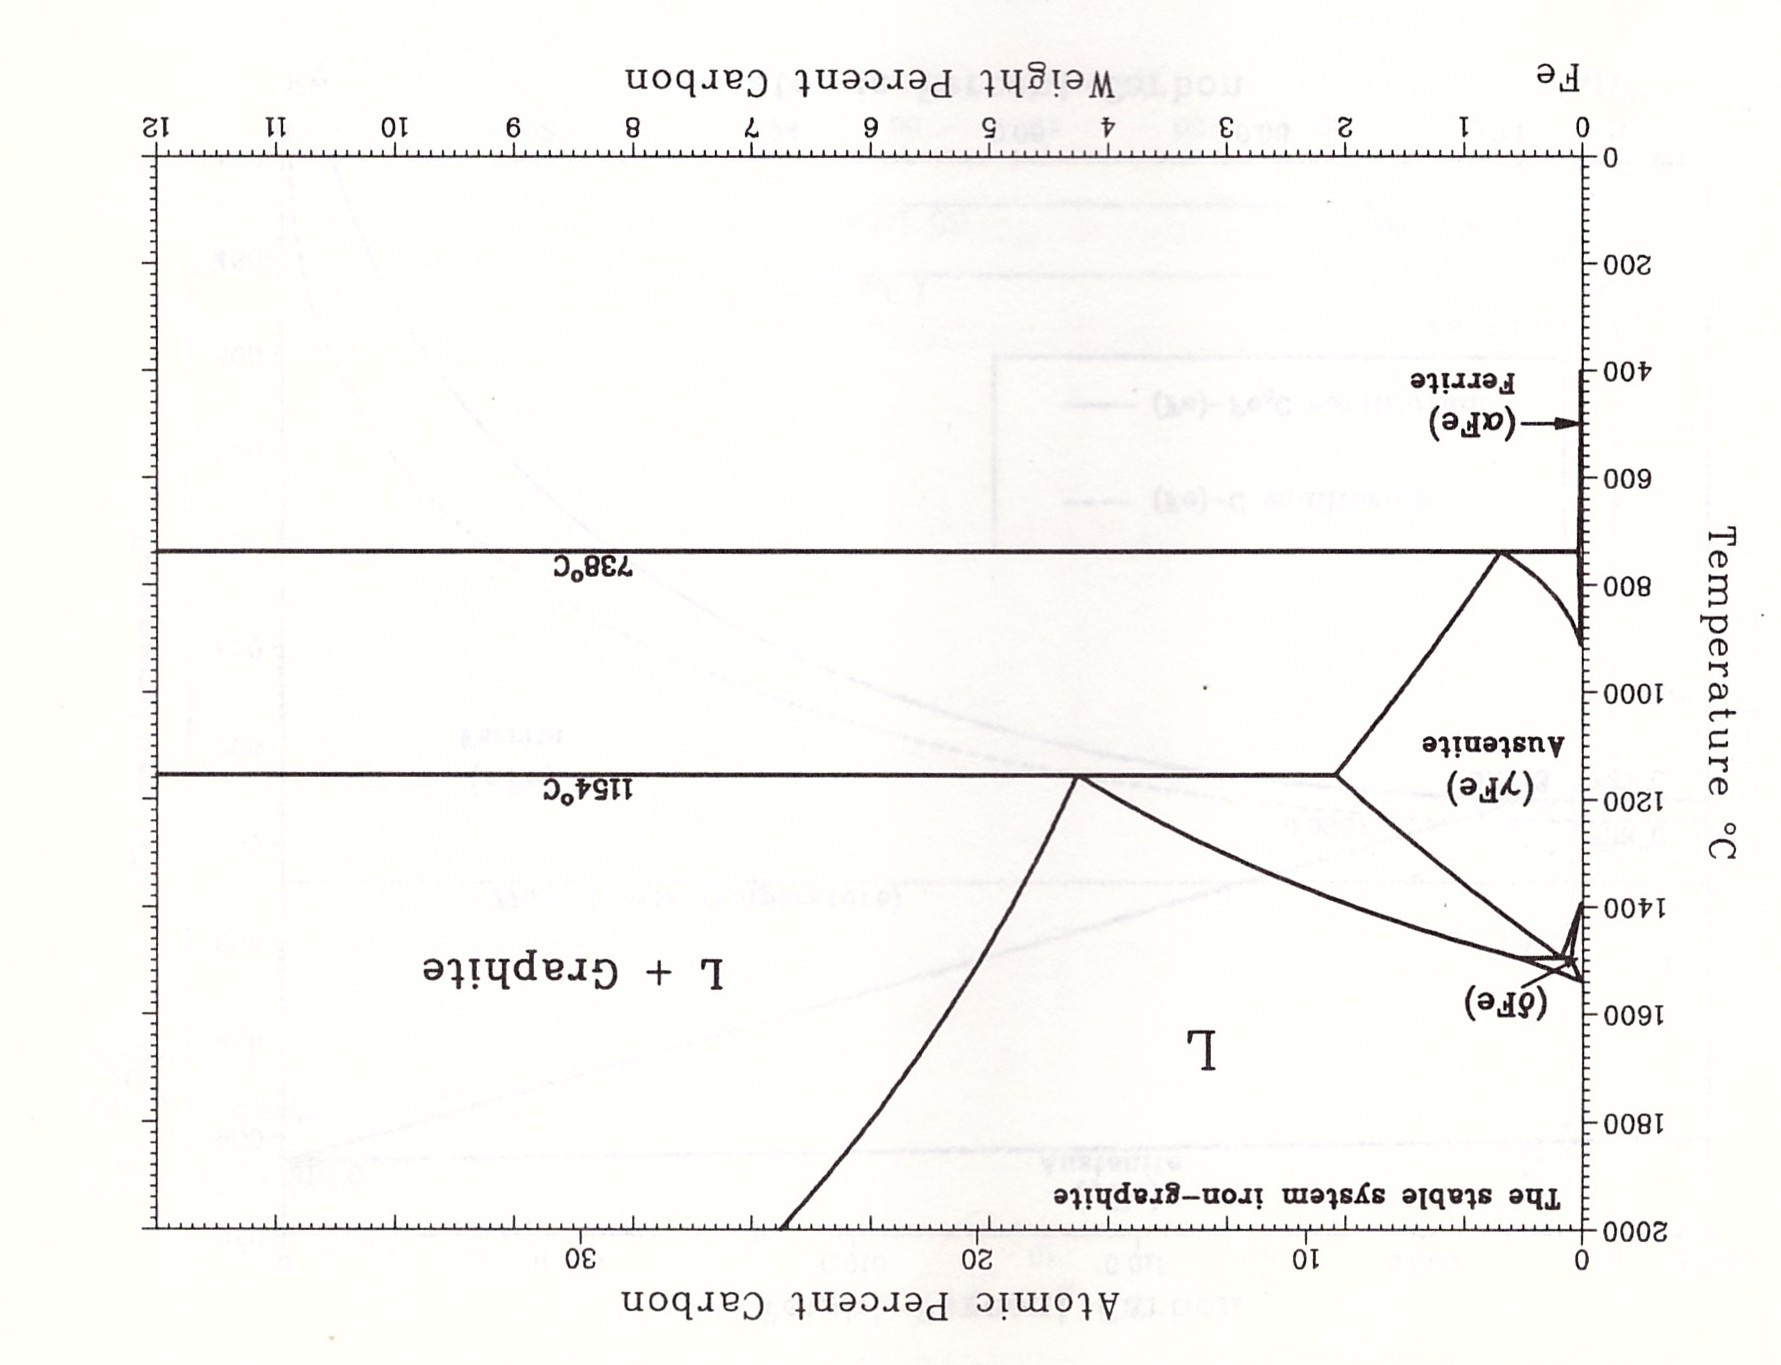
\includegraphics[width=.8\textwidth,angle=180]{img/Fe-C.jpg}
  \caption{Diagrama de equilíbrio ferro-carbono \cite{Massalski1996v1}}
  \label{fig:diagrama_fe-c}
\end{figure}

Entretanto a condição de equilíbrio não é verificada para a maioria dos processos e, em vez de grafita, forma-se o carboneto de ferro \ch{Fe3C}, também chamado de cementita. A cementita é uma fase metaestável, mas sua formação é favorecida cineticamente em relação à grafita devido às elevadas taxas de resfriamento aplicadas ao aço durante seu processamento.
% uma vez que a solidificação e resfriamento do aço são muito rápidos.
% , que apesar de ser uma fase metaestável pode ser considerada estável, pois o coeficiente de difusão do carbono no ferro é muito baixo (\SI{2,9e-19}{cm^2/s}).
Para essas condições, o diagrama de fase, que é então chamado de diagrama de equilíbrio metaestável, é dado pela Figura \ref{fig:diagrama_fe-c_meta}.

\begin{figure}[ht!]
  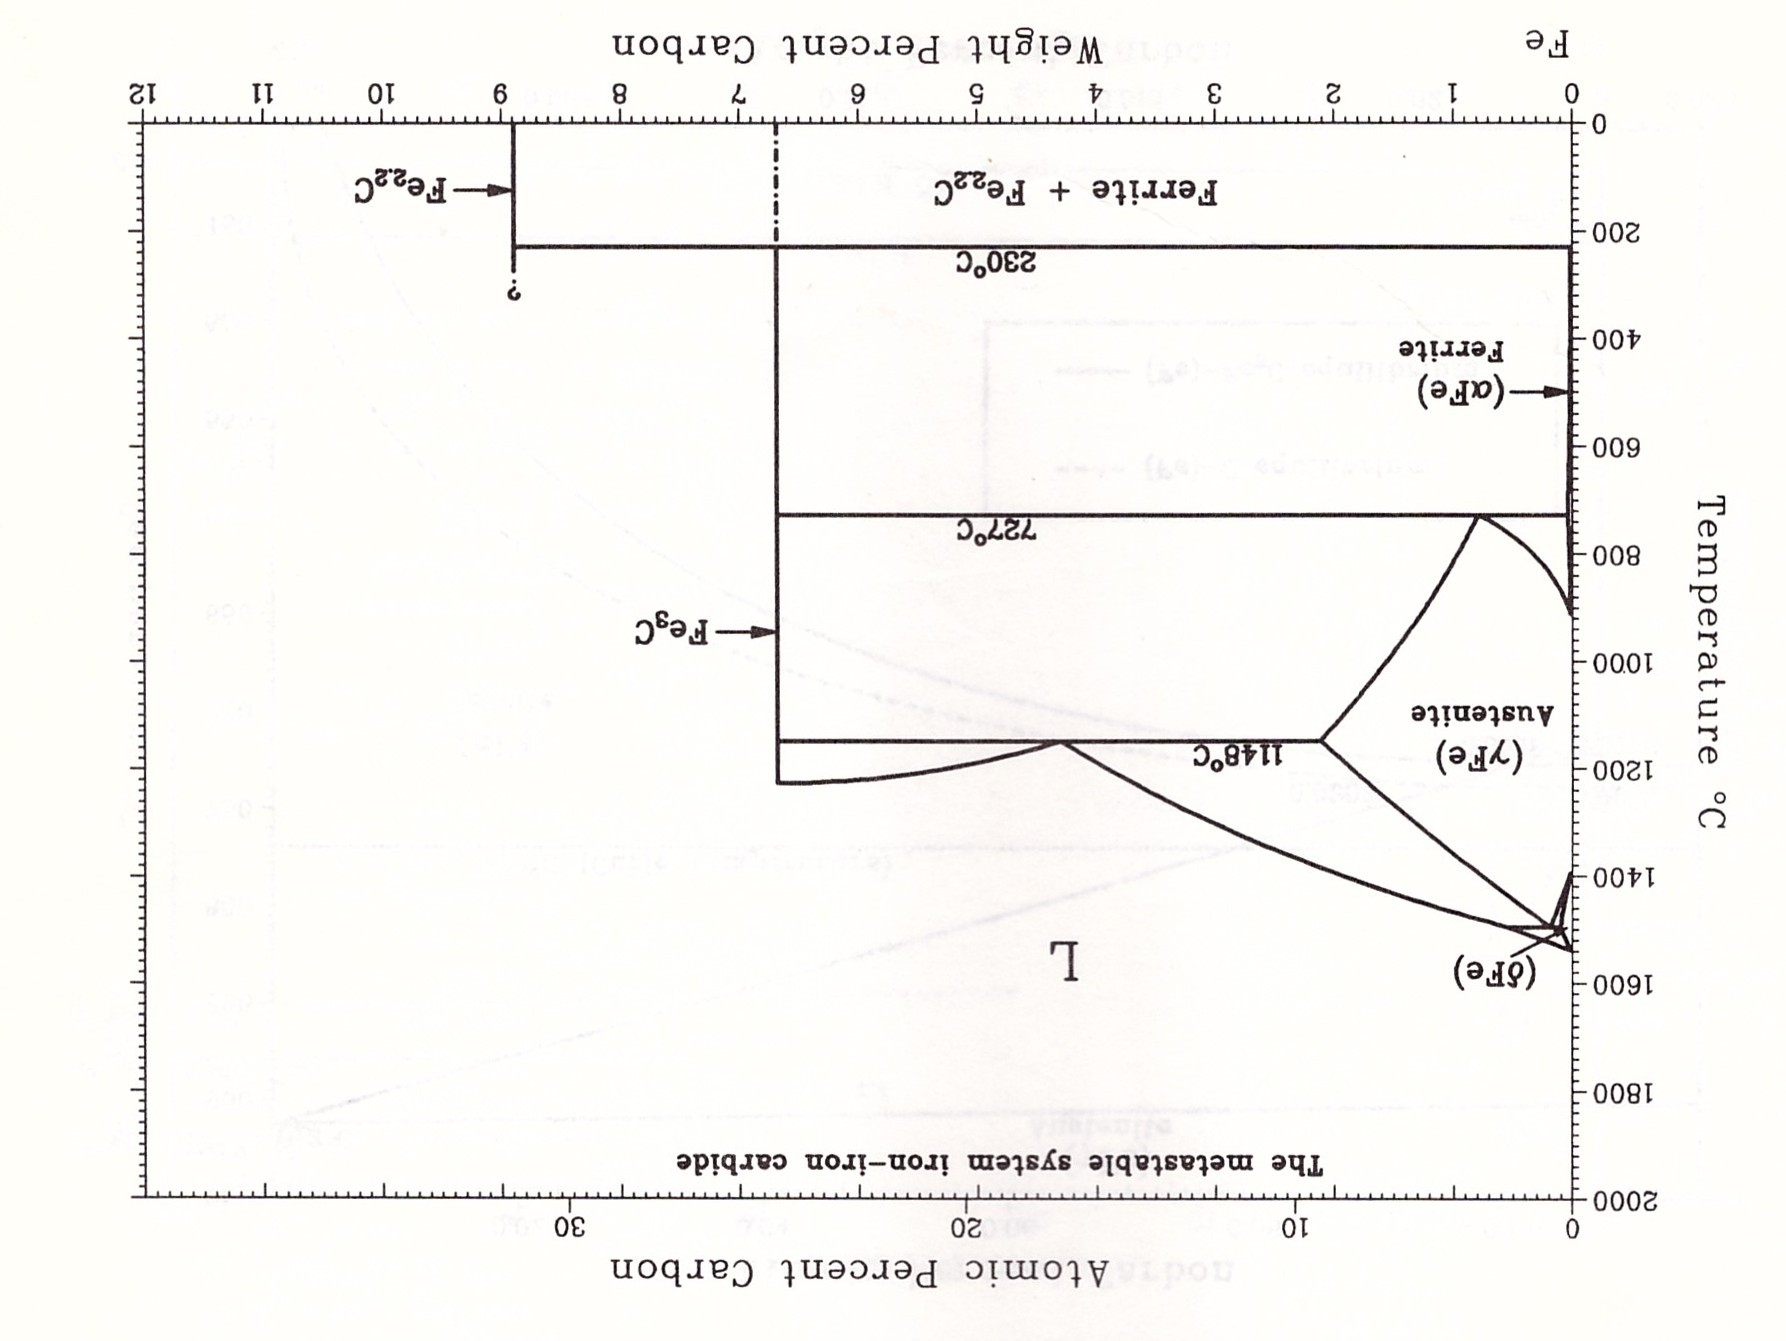
\includegraphics[width=.8\textwidth,angle=180]{img/Fe-C_meta.jpg}
  \caption{Diagrama de fases metaestável ferro-carbono \cite{Massalski1996v1}}
  \label{fig:diagrama_fe-c_meta}
\end{figure}

Um ponto importante do diagrama é o ponto eutetóide, no qual as três fases coexistem. Para um sistema apenas ferro e carbono, ele corresponde a aproximadamente 0,8\% C em massa. Assim, aços de composição abaixo desse ponto são denominados hipoeutetóides e, acima, hipereutetóides.

\section{Decomposição da Austenita}

Para um aço resfriado lentamente à temperatura ambiente, o teor de carbono controla as fases formadas. Entretanto, a taxa de resfriamento controla a formação de constituintes metaestáveis. Essa formação de constituintes a partir da austenita pode ocorrer por difusão, cisalhamento ou uma mistura dos dois mecanismos \cite{Honeycombe1982}.

No caso da ferrita, o resfriamento lento resulta em grãos equiaxiais preferencialmente no contorno de grão austenítico, enquanto um resfriamento rápido gera grãos em forma de agulhas, também conhecidos como ferrita acicular, nucleados no contorno e no interior do grão austenítico  \cite{Silva2010} %{Krauss1997}apud{Silva2010} ARRUMAR.
A cementita segue o mesmo comportamento morfológico e ambas ocorrem sob mecanismo exclusivo de difusão \cite{Honeycombe1982}.

Para um aço de composição eutetóide, o resfriamento lento produz perlita, uma microestrutura característica que na realidade é uma mistura de austenita e cementita, na forma de lamelas. A ferrita é menos compacta por ter estrutura CCC e, consequentemente, apresenta insterstícios tetraédricos menores. Assim, à medida que o resfriamento ocorre, o carbono da austenita é rejeitado pela ferrita em formação, dando origem à cementita, fase rica em carbono \cite{Silva2010}.

Já um aço carbono resfriado bruscamente produz a martensita, uma estrutura que mantém o carbono em solução sólida da austenita. Diferente da formação de ferrita e perlita, esse processo não é controlado pela difusão devido à sua condição de resfriamento, mas sim por uma distorção na rede. Dessa forma, é um constituinte de mesma composição da austenita. Ela é característica pela sua microestrutura em ripas e alta dureza \cite{Honeycombe1982}.

Já a bainita é um constituinte intermediário, pois reúne o rearranjo de rede da martensita à redistribuição de carbono e precipitação de carboneto da perlita \cite{Totten2006}. Sua natureza se modifica com a diminuição da temperatura de transformação, sendo classificada em bainita superior e inferior. A morfologia da bainita superior contem ferrita na forma de ripas, de concentração de carbono muito inferior à da austenita mãe; já a cementita depende do teor de carbono, podendo assumir a forma de partículas isoladas ou mesmo não precipitar, permanecendo na forma de austenita retida. Já a bainita inferior é mais acicular e tem lamelas mais individualizadas \cite{Honeycombe1982}.

\section{Temperaturas cr\'iticas de aços}

O francês Le Chatelier foi o primeiro a atribuir a letra ``A'' para as temperaturas críticas de transformação, devido à palavra \textit{Arrêt}, que representa a parada na temperatura durante a transformação de fase \cite{Silva2010}.

Para exemplificar essas temperaturas críticas em aços, utilizou-se dados de chamadas do software Thermo-Calc\textregistered{} para traçar o diagrama Fe-C metaestável para um aço 1\% Mn, em massa, da Figura \ref{fig:fe-1mn-C_isopleth}, bem como os gráficos de fração molar de fase em função da temperatura para aços hipo, hiper e eutetóide, das Figuras \ref{fig:fe-01c-1mn}, \ref{fig:fe-0727c-1mn} e \ref{fig:fe-1c-1mn} a seguir.

\begin{figure}[ht!]
  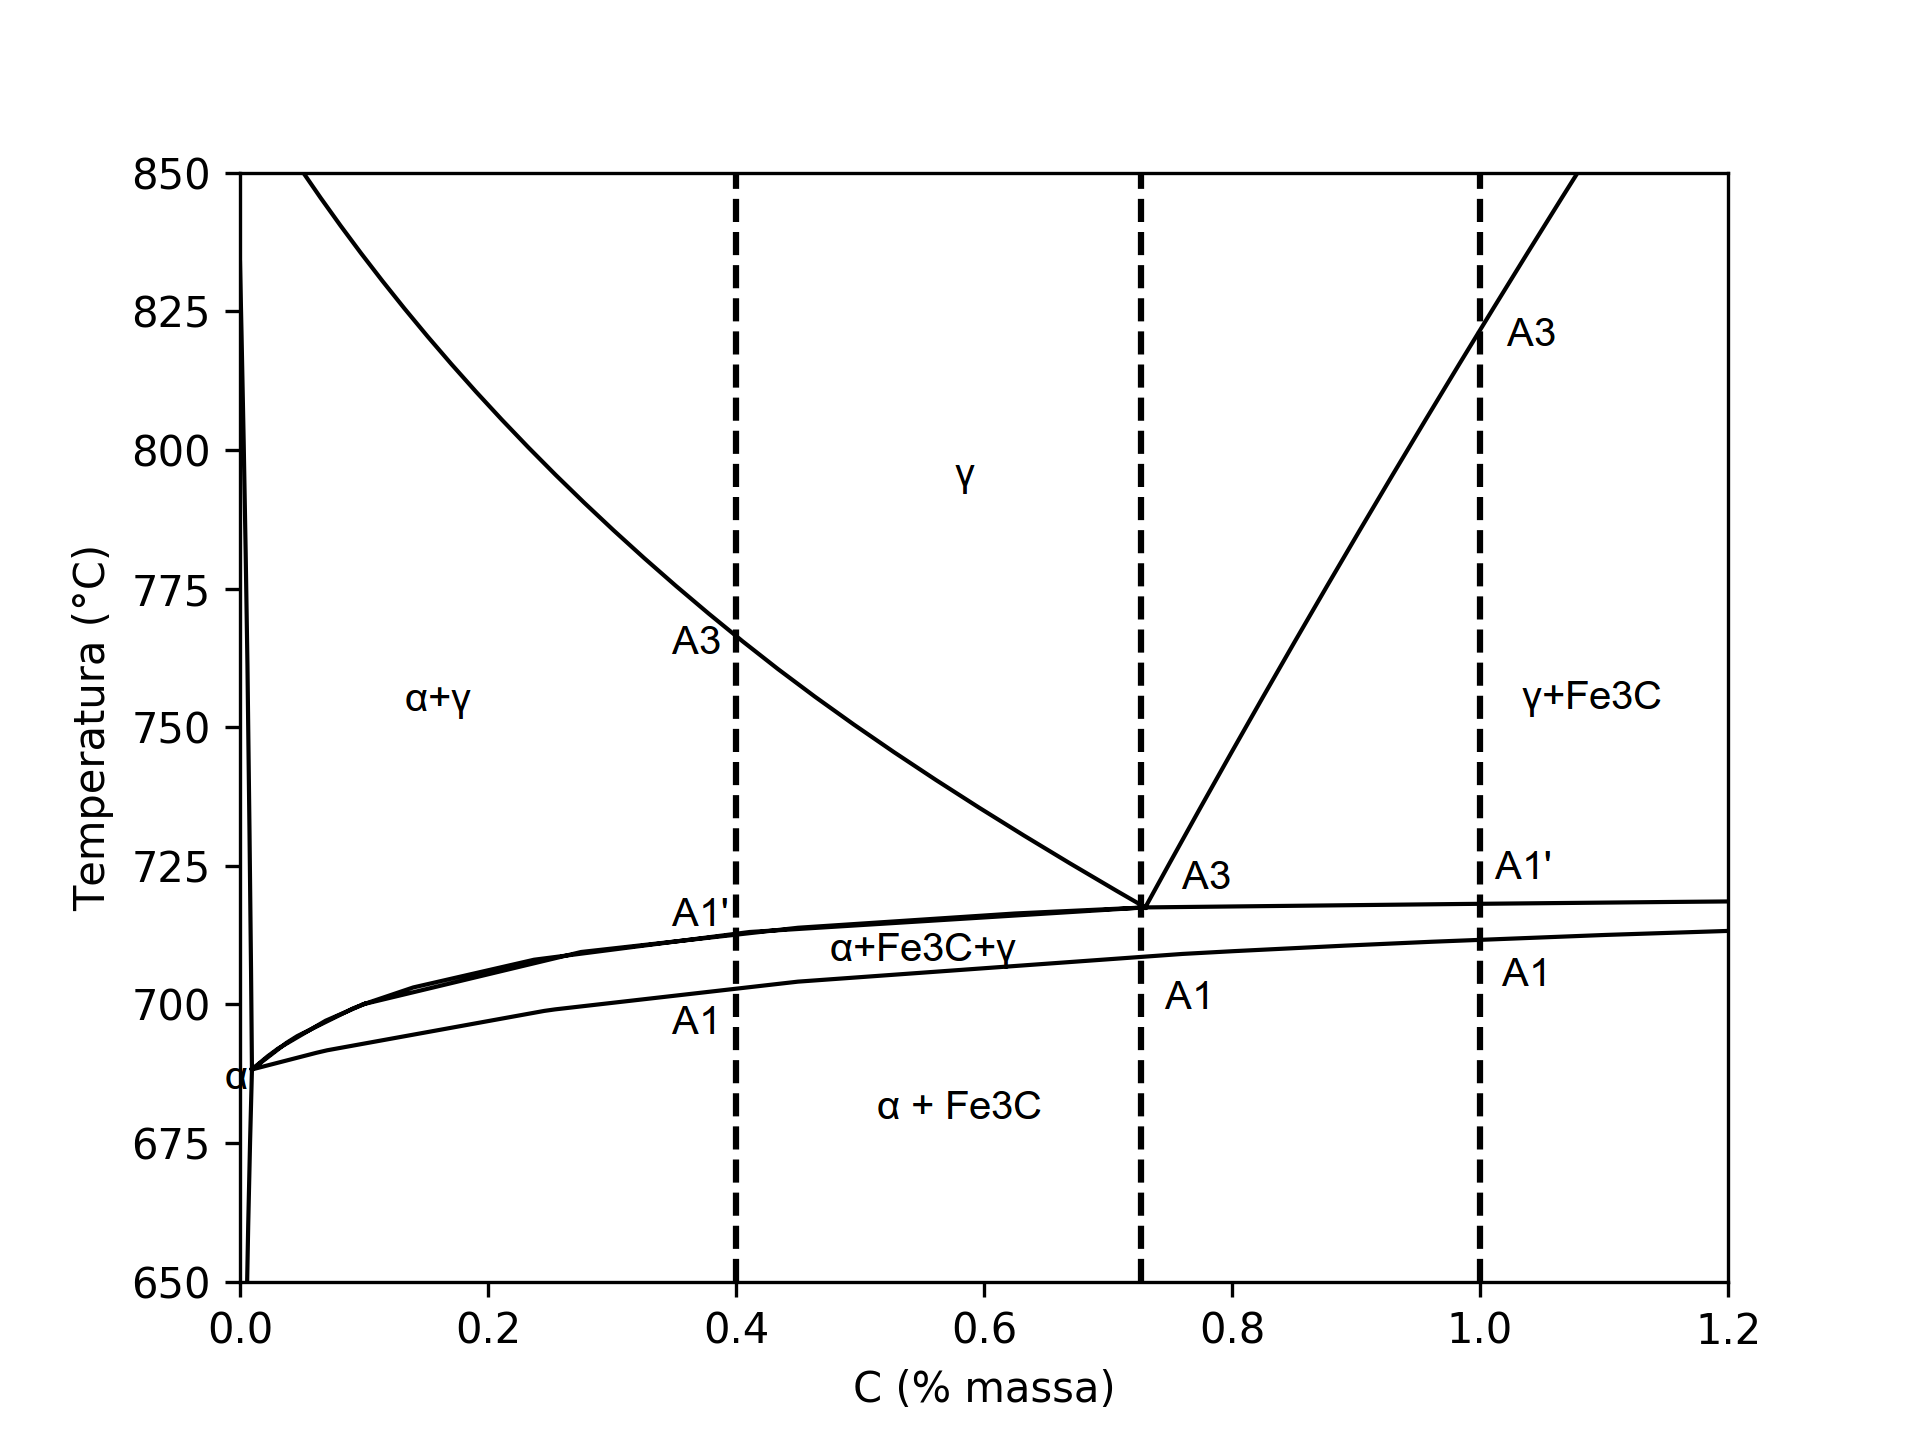
\includegraphics[width=.9\textwidth]{img/Fe-1Mn-C_isopleth_edited.png}
  \caption{Diagrama de fases Fe-C para aço 1\% Mn, em massa}
  \label{fig:fe-1mn-C_isopleth}
\end{figure}

A primeira linha vertical tracejada da Figura \ref{fig:fe-1mn-C_isopleth} representa um aço hipoeutetóide e sua fração molar de fases pode ser vista na Figura \ref{fig:fe-01c-1mn}.

\begin{figure}[ht!]
  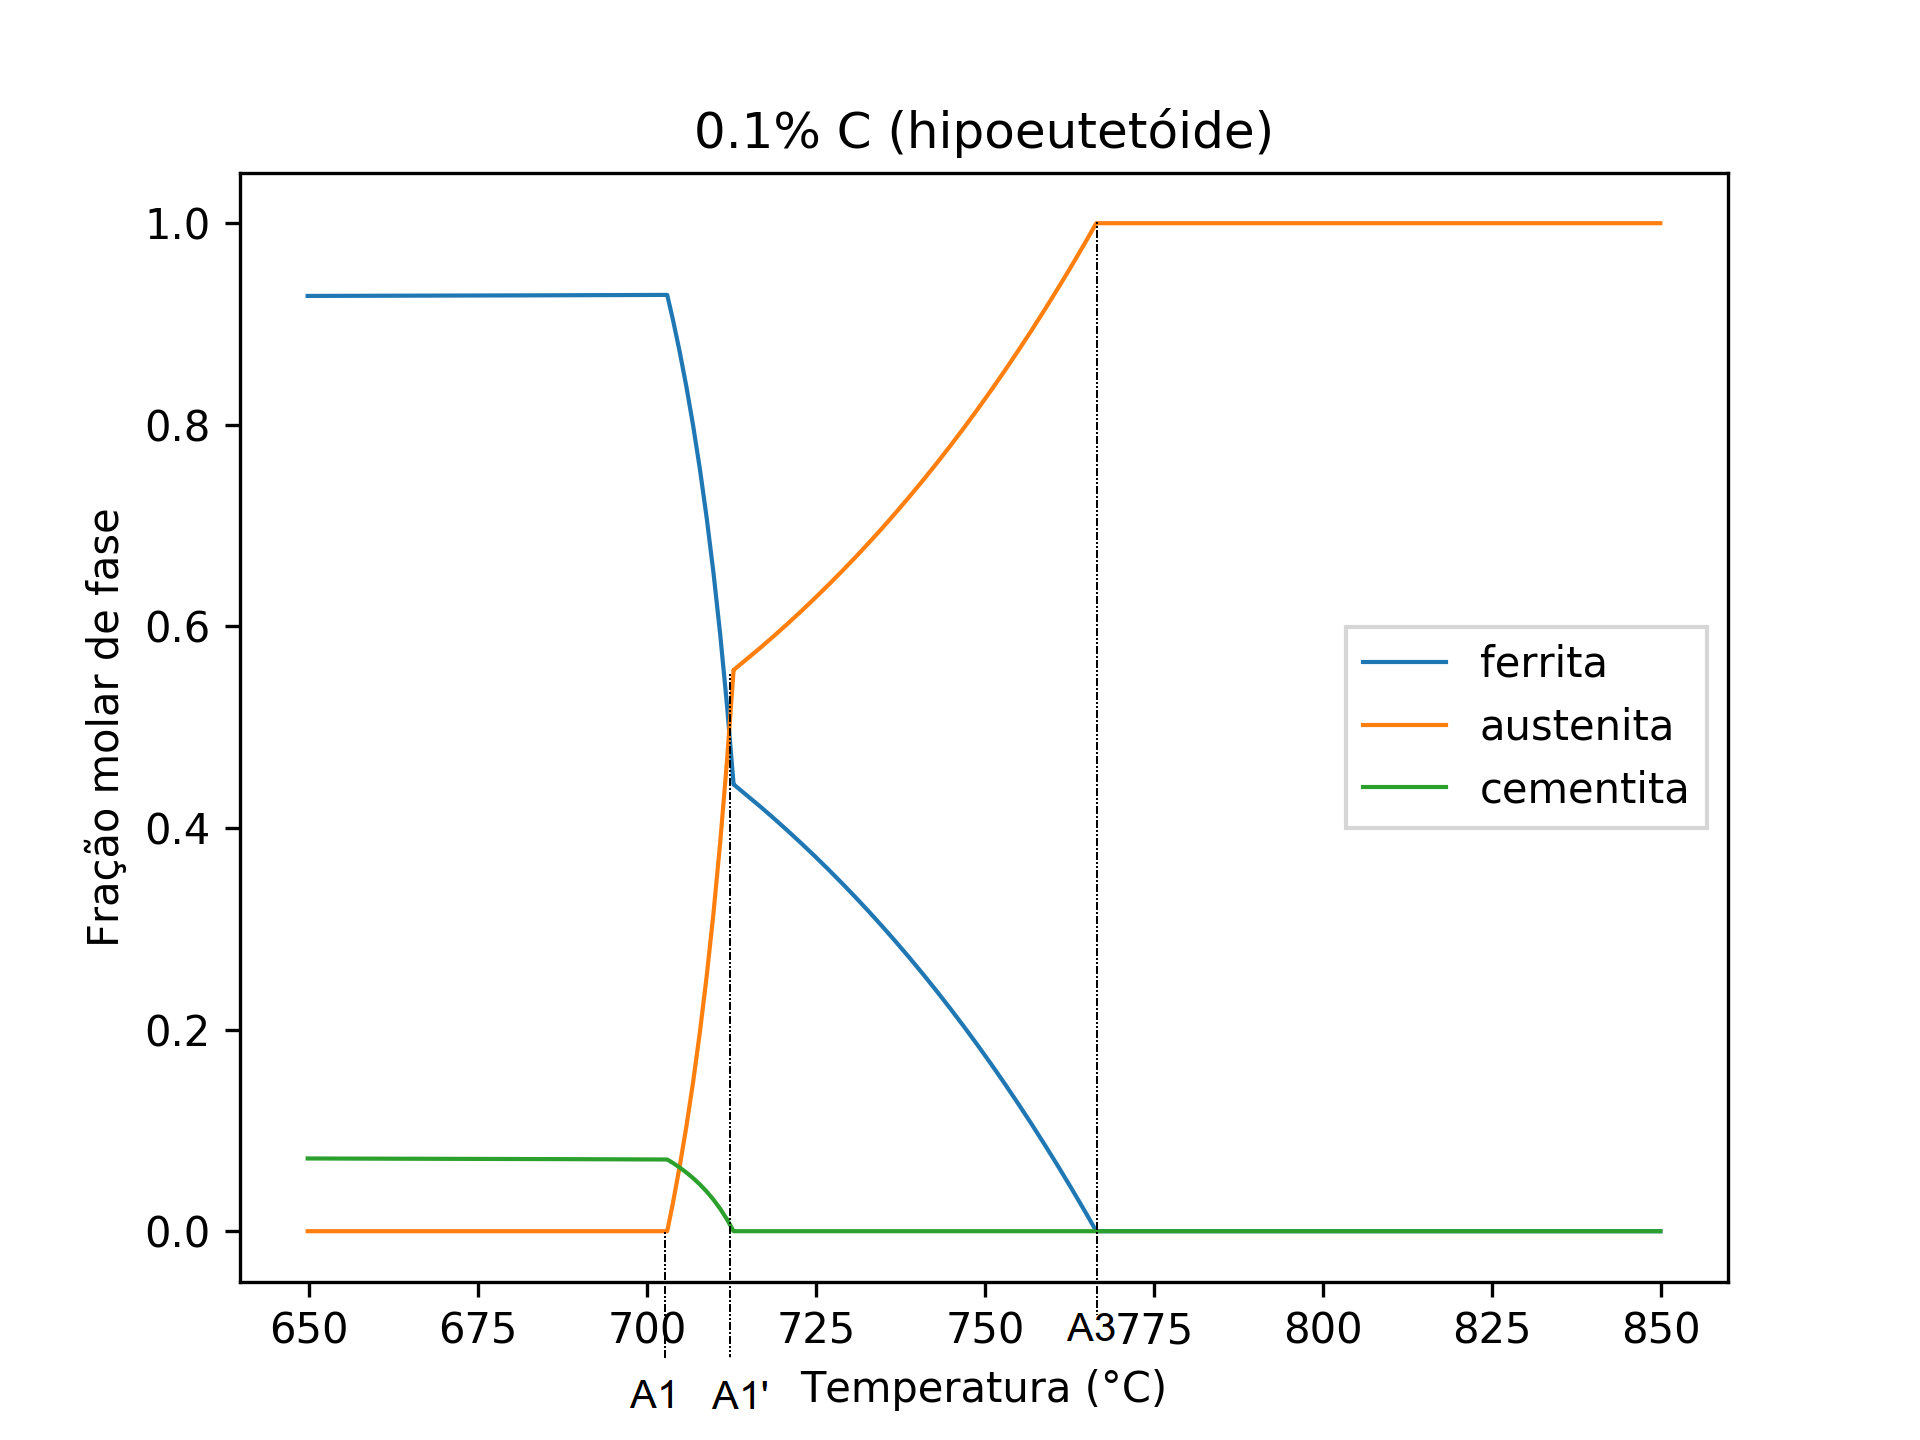
\includegraphics[width=1.1\textwidth]{img/Fe-Mn-01C_edited.png}
  \caption{Fração molar de fase versus Temperatura para aço 0,1\%C 1\% Mn, em massa}
  \label{fig:fe-01c-1mn}
\end{figure}

Um aço nessa composição, mediante aquecimento, mantém as fases $\alpha$ e \ch{Fe3C} até chegar ao ponto A1, no qual a fase $\alpha$ começa a se decompor em $\gamma$. No gráfico da Figura \ref{fig:fe-01c-1mn}, esse ponto pode ser notado pela primeira mudança de inclinação da curva da austenita. O aço permanece no campo trifásico até encontrar o ponto A1', quando toda a fase \ch{Fe3C} se transforma em $\gamma$, a segunda mudança de inclinação na curva da austenita. Caso o aquecimento permaneça, a fase $\alpha$ começa a se transformar em $\gamma$, até atingir o ponto A3, onde tem-se 100\% de fase $\gamma$, a última mudança de inclinação na curva da austenita.

Um aço eutetóide, correspondente à segunda linha vertical tracejada da Figura \ref{fig:fe-1mn-C_isopleth} e ao gráfico da Figura \ref{fig:fe-0727c-1mn}, segue o mesmo raciocínio. A diferença é que não há um campo trifásico, por isso a temperatura A1' equivale à temperatura A3.

\begin{figure}[ht!]
  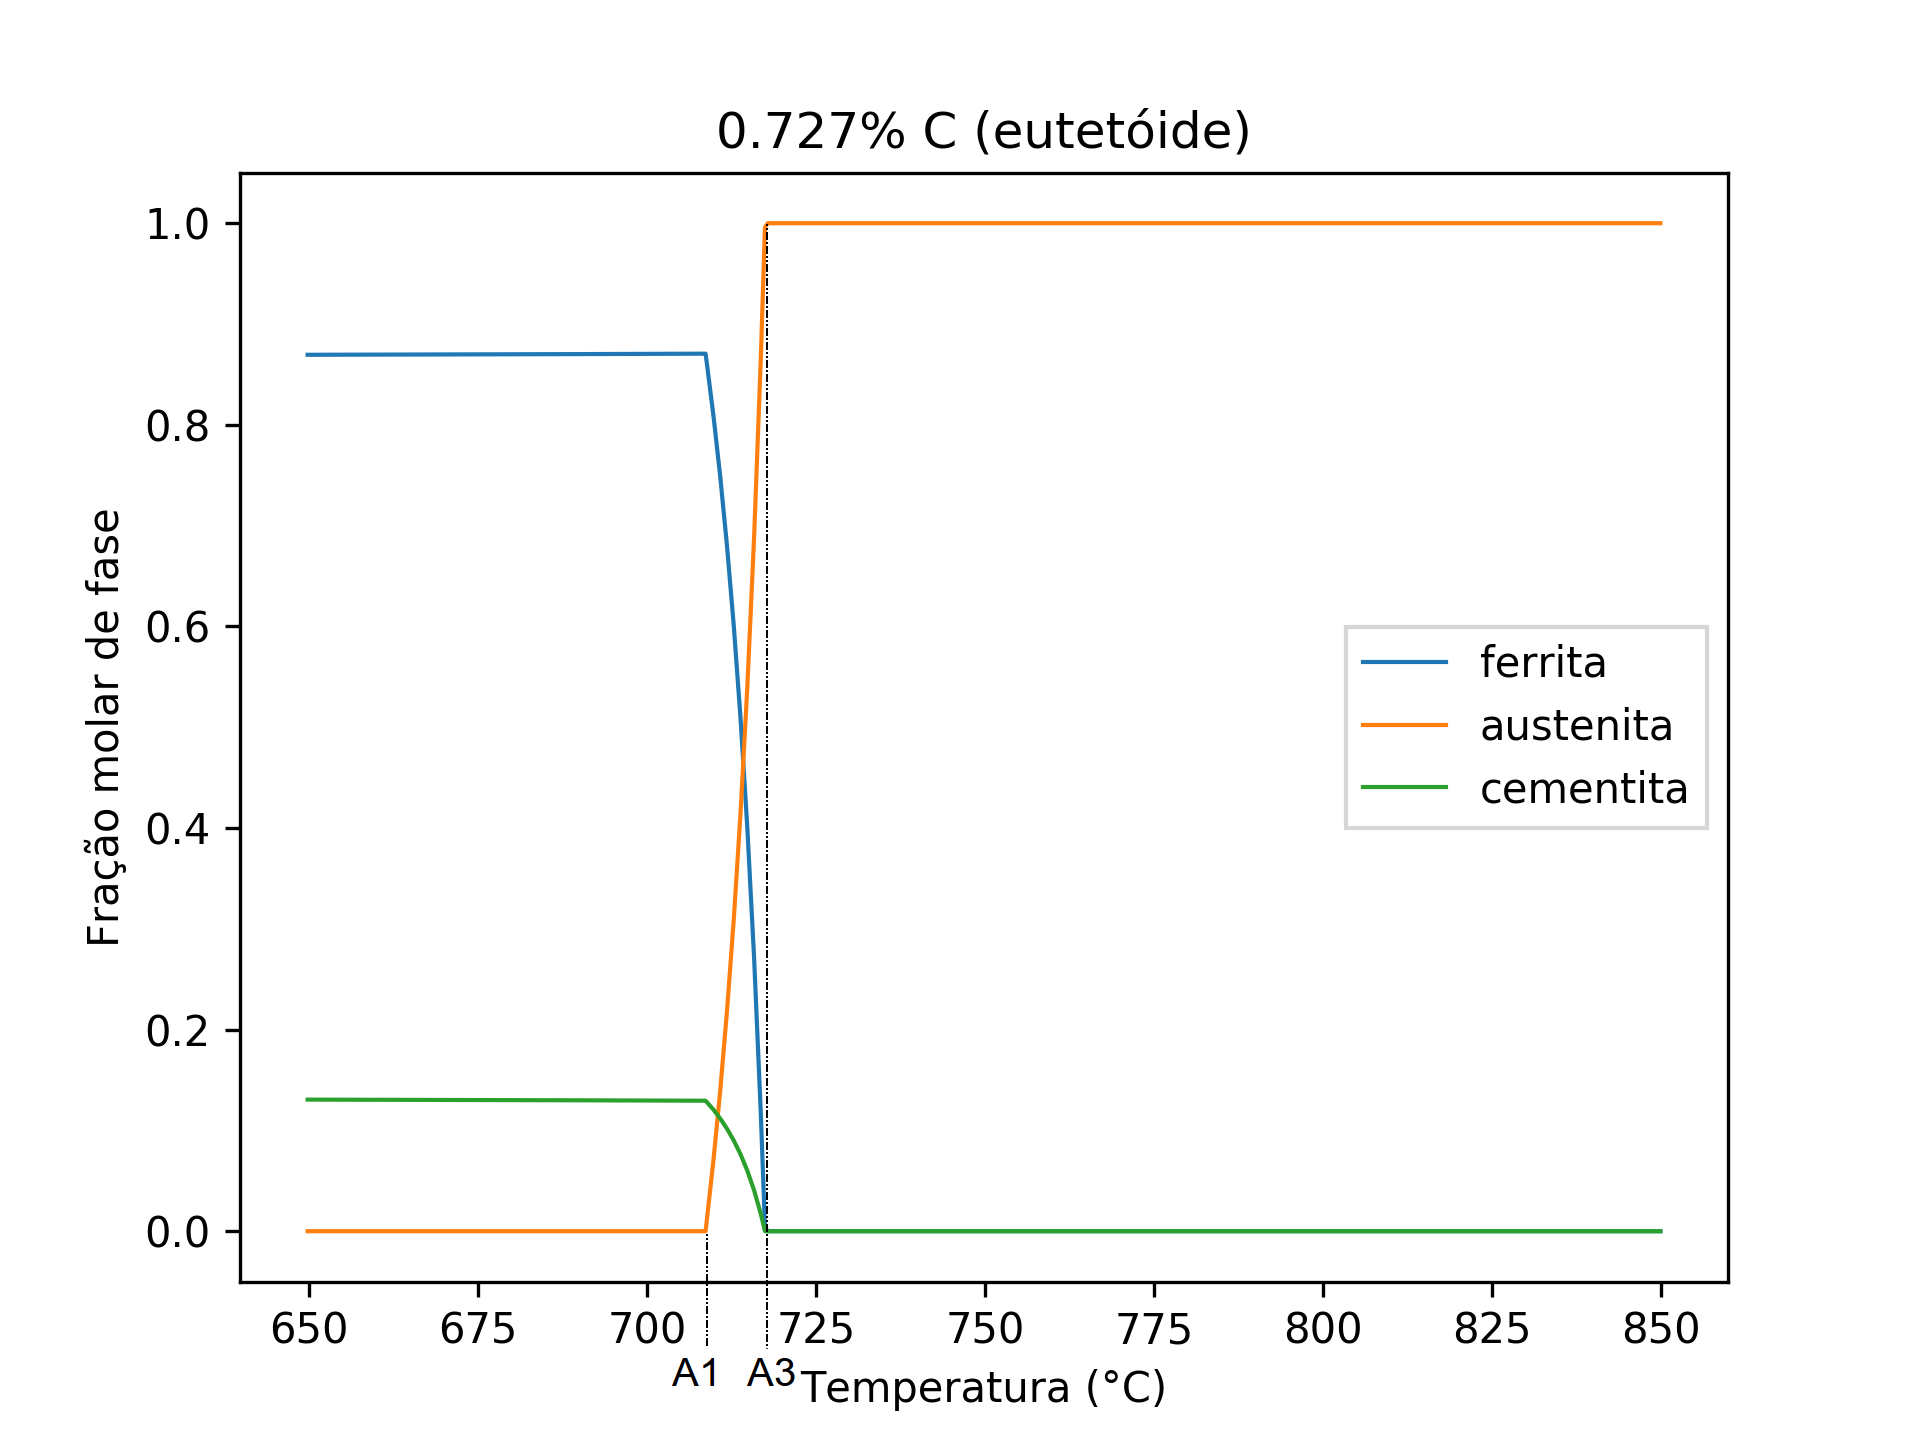
\includegraphics[width=1.1\textwidth]{img/Fe-Mn-0727C_edited.png}
  \caption{Fração molar de fase versus Temperatura para aço 0,727\%C 1\% Mn, em massa}
  \label{fig:fe-0727c-1mn}
\end{figure}

Já para um aço hipereutetóide, terceira linha vertical tracejada da Figura \ref{fig:fe-1mn-C_isopleth} e gráfico da Figura \ref{fig:fe-1c-1mn}, a diferença é que o segundo campo bifásico é constituído por $\gamma$ e \ch{Fe3C}, até atingir o ponto em que toda a \ch{Fe3C} se transforma em $\gamma$. Certas literaturas, como \citaremsentenca{Digges1960}, fazem distinção para a temperatura A3 de aços hipereutetóides, chamando-a de Acm, devido à diferença de campos bifásicos. No presente trabalho, ambas serão chamadas de A3, por corresponderem à mínima temperatura em que a fração de austenita é igual a 1.

\begin{figure}[ht!]
  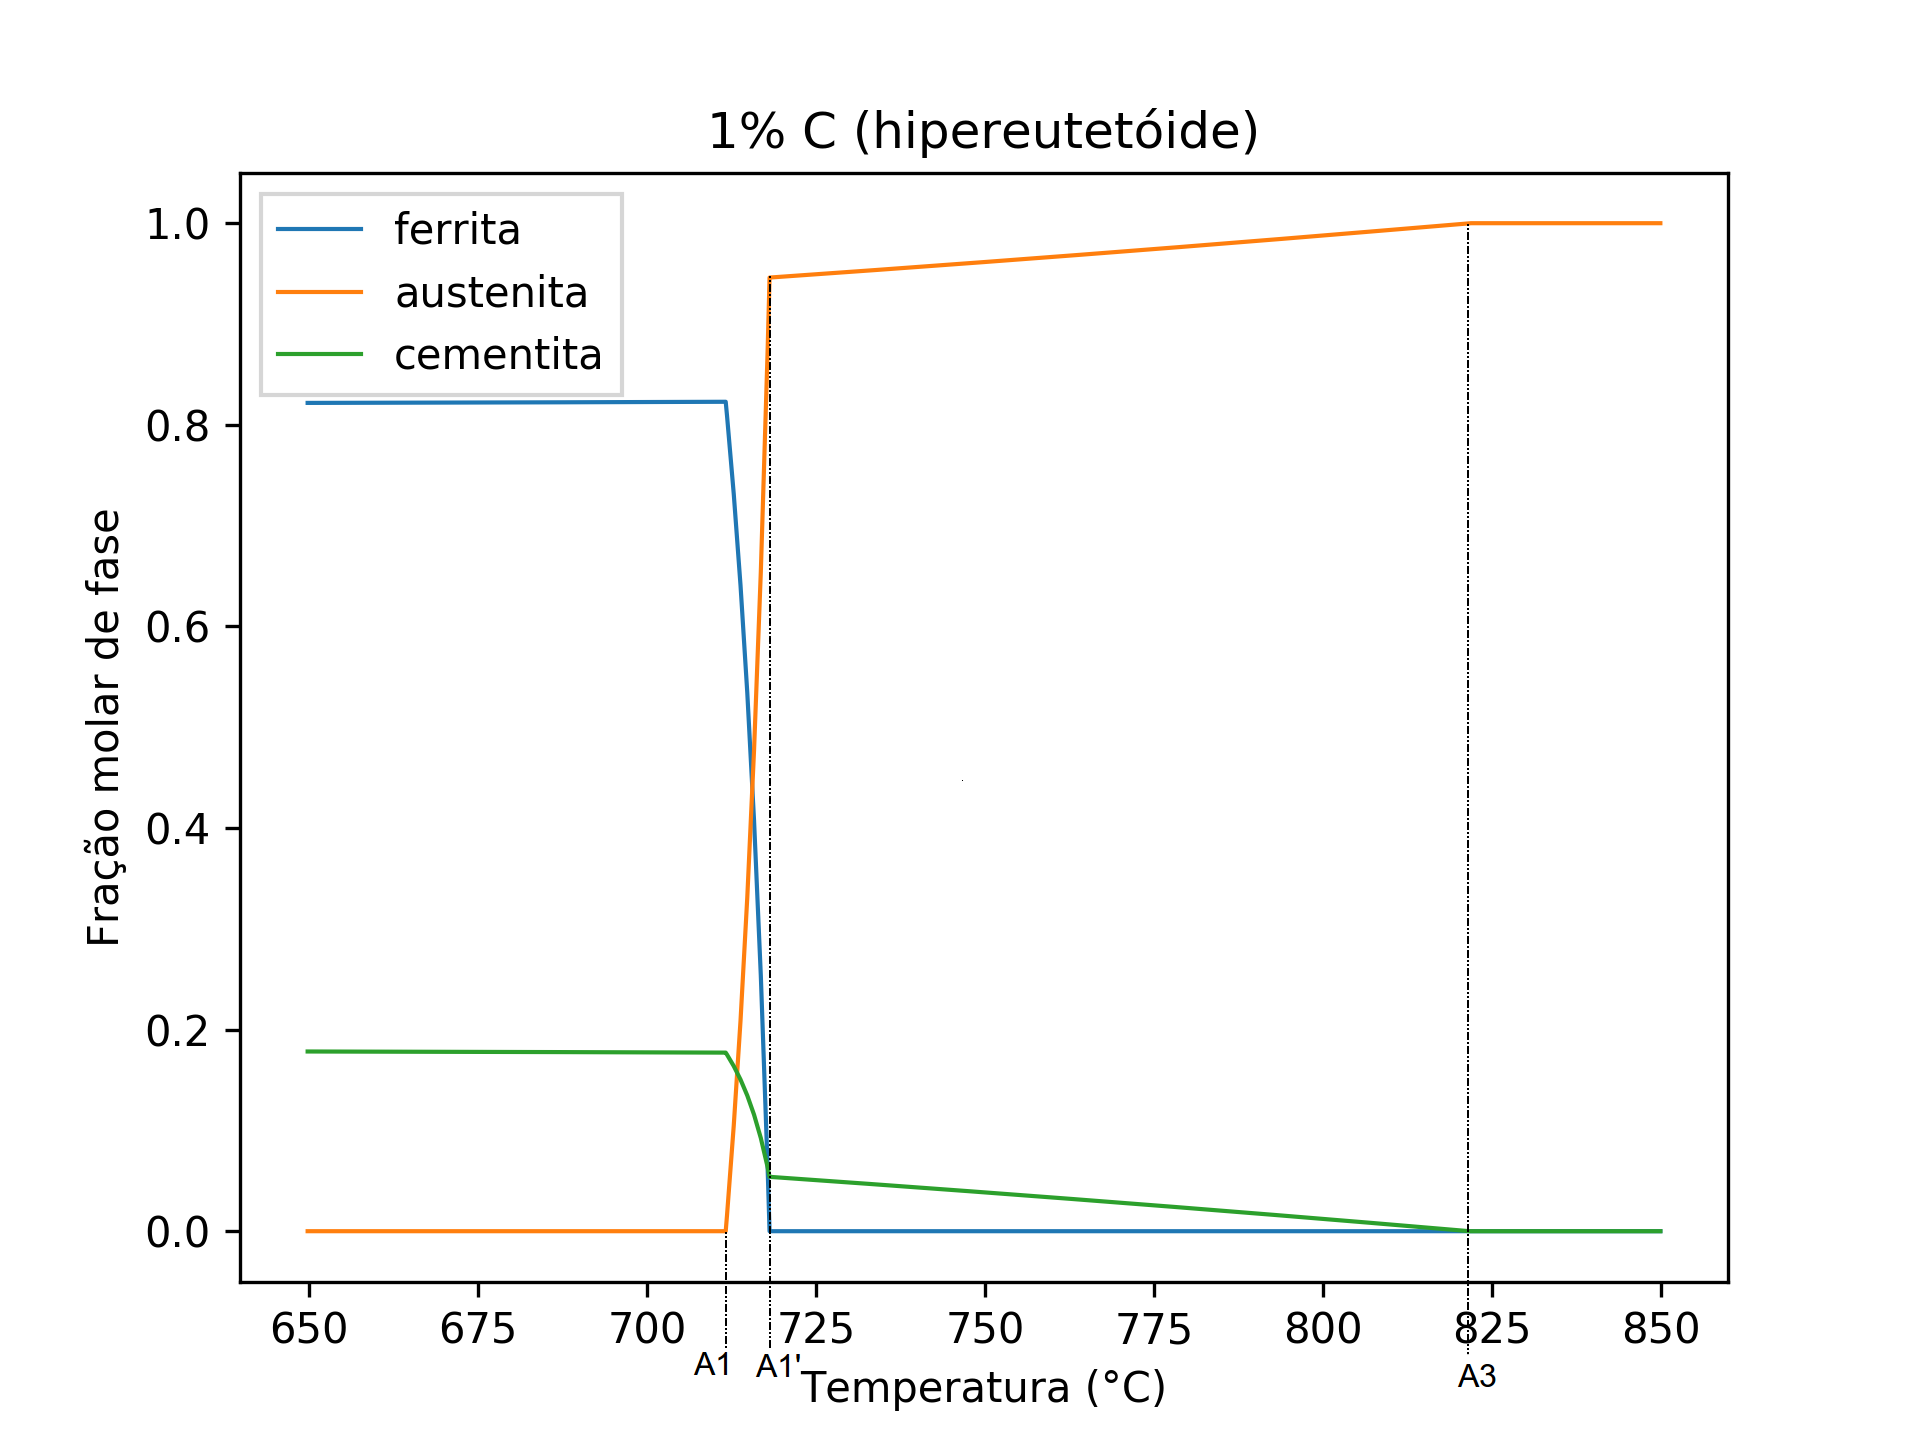
\includegraphics[width=1.1\textwidth]{img/Fe-Mn-1C_edited.png}
  \caption{Fração molar de fase versus Temperatura para aço 1\%C 1\% Mn, em massa}
  \label{fig:fe-1c-1mn}
\end{figure}

Em resumo, pode-se dizer que a temperatura A1 corresponde à máxima temperatura em que a fração de austenita é zero, enquanto a A3 é a mínima temperatura cuja fração de austenita é um e A1' é o limite superior do campo intercrítico de três fases \cite{Honeycombe1982}.

É possível ainda diferenciar a temperatura crítica no resfriamento da de aquecimento, utilizando respectivamente as letras ``r'' e ``e''. Em teoria, elas deveriam ser iguais, mas na prática a taxa de resfriamento ou aquecimento diferencia Ae1 de Ar1 e Ae3 de Ar3. A faixa de temperatura entre A1 e A3 é chamada de intervalo crítico ou de transformação \cite{Digges1960}.

\section{Tratamento térmico de aços}

A obtenção das propriedades ideais de um aço está relacionada tanto com sua composição química quanto com os processos de tratamento térmico aos quais ele é submetido \cite{Totten2006}. Tratamentos térmicos podem ser utilizados para aumentar ou diminuir a ductilidade, dureza, tensão de escoamento ou tenacidade, otimizando essas propriedades para a finalidade do material \cite{Silva2010}.

A austenitização é a etapa que precede um tratamento térmico e consiste em aquecer o aço a uma temperatura em que haja formação da austenita. Esta pode ser parcial, quando se encontra na faixa de transformação, ou total, quando está acima do intervalo de transformação \cite{ASM1991}.

%RECOZIMENTO
A partir do aço na forma de austenita, é possível fazer o recozimento, ou seja, o resfriamento lento para reduzir tensões, diminuir dureza, melhorar a usinabilidade ou ajustar o tamanho do grão, reduzindo assim influências de tratamentos térmicos ou mecânicos anteriores. Para aços hipoeutetóides a temperatura é de aproximadamente \SI{50}{\celsius} acima de A3, enquanto para hipereutetóides é de \SI{50}{\celsius} acima de A1, não podendo ultrapassar A3 pois em um resfriamento posterior formaria cementita nos contornos de grão da austenita, fragilizando a peça tratada. Quando se deseja uma estrutura perlítica, prefere-se temperaturas de austenitização mais altas, e mais baixas para estrutura esferoidizada. Para ambos os casos, quanto mais próxima de A1 for a temperatura de transformação da austenita, mais grosseira será a estrutura .

%NORMALIZAÇÃO
Outro tipo de tratamento térmico é a normalização, que após austenitização resfria lentamente o aço ao ar parado ou agitado, sendo recomendada para homogeneizar a estrutura após forjamento ou antes de outros processos, como têmpera ou revenimento. Em aços hipoeutetóides, causa um espaçamento entre as lamelas da perlita, tornando-a mais fina. A dureza e a resistência mecânica ficam mais elevadas e a dutilidade mais baixa. Para hipereutetóides, distribui-se melhor os carbonetos, pois a temperatura de austenitização ocorre acima de A3.

%TÊMPERA
Um terceiro tipo de processo muito importante é a têmpera, que consiste em resfriar o aço austenitizado rapidamente a fim de obter a estrutura metaestável martensítica. O teor de carbono aumenta a dureza da martensita e diminui a temperatura necessária para que o processo ocorra. Essa temperatura depende não só da composição do aço, mas também da taxa de resfriamento, e é chamada de Ms. Por depender de fatores cinéticos, essa temperatura crítica não será o foco do presente trabalho.

%REVENIMENTO
A formação de martensita aumenta a dureza do aço, entretanto o torna mais frágil. Para  melhorar a resistência mecânica e tenacidade do material temperado, realiza-se o revenimento da martensita, aquecendo o aço até temperatura inferior à de austenitização, mantendo-a até que as propriedades desejadas sejam alcançadas \cite{Silva2010}. Como a martensita é uma solução supersaturada de carbono, durante o revenimento o ferro o rejeita na forma de carbonetos em uma matriz de ferro $\alpha$ \cite{Honeycombe1982}.

\section{Efeito dos elementos de liga nas temperaturas críticas e tratamento térmico}
%INSERIR DIAGRAMAS BINÁRIOS
Os elementos de liga são adicionados ao aço para modificar as fases ou constituintes em equilíbrio, bem como alterar a maneira como essas fases se formam \cite{Silva2010}.

Quanto maior o teor de carbono, maior a temperabilidade do aço. Entretanto, esse também fica mais suscetível a trincas durante a têmpera. Assim, a adição de elementos de liga tem como um de seus objetivos manter a alta temperabilidade do aço com baixa suscetibilidade a trincas, através da transaformação da austenita em menor velocidade \cite{Souza1989}.

Os elementos de liga são classificados em dois tipos: os estabilizadores de austenita e os estabilizadores de ferrita.

\section{Determinação das Temperaturas Críticas}

Dada a importância de conhecer as temperaturas críticas de aços para obtenção das propriedades desejadas, foram desenvolvidas diversas formas para determiná-las.

Como as transformações de fase do aço também causam contração ou expansão, um método de determinação experimental é através da dilatometria sob aquecimento contínuo. O dilatômetro coleta sinais de mudança nas dimensões do corpo de prova bem como sua temperatura, para traçar a curva de derivada da dimensão relativa em função da temperatura, como as do exemplo na Figura \ref{fig:dilatometer}. Na literatura utilizada por \citaremsentenca{Pawlowski2012}, A1 equivale a A\textsubscript{c1p}, A1' a A\textsubscript{c1k}, e A3 a Ac\textsubscript{3} ou Acm. Apesar de muito preciso, o equipamento tem custo elevado e necessita de pessoas capacitadas para operá-lo.

\begin{figure}[ht!]
  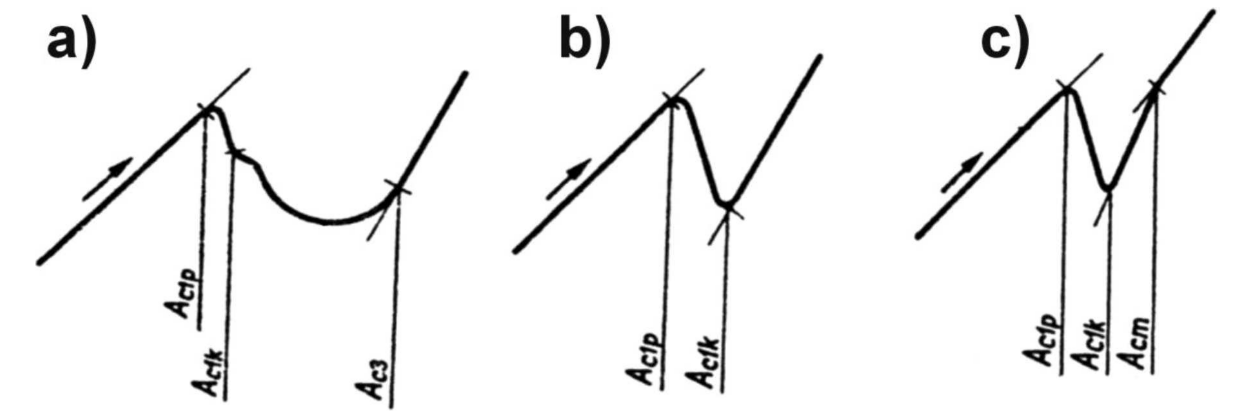
\includegraphics[width=.9\textwidth]{img/dilatometer.png}
  \caption{Determinação gráfica das temperaturas críticas em aço (a) hipoeutetóide, (b) eutetóide e (c) hipoeutetóide, a partir de dados do dilatômetro \cite{Pawlowski2012}}
  \label{fig:dilatometer}
\end{figure}

Outro método de determinar as temperaturas críticas de transformação é através do Thermo-Calc\textregistered{}, software utilizado para diversos cálculos termodinâmicos baseado na minimização da energia de Gibbs. Ele tem acesso a diversos bancos de dados termodinâmicos, em especial os desenvolvidos pelo \textit{Scientific Group Thermodata Europe} (SGTE). Sendo um resultado de mais de 30 anos de coleta de dados, sua precisão é inquestionável \cite{TC2002}. Entretanto, trata-se de um software pago e requer certo aprendizado para sua manipulação.

Uma terceira maneira é a utilização de equações empíricas que se baseiam na concentração em massa dos elementos presentes no aço. A elaboração dessas equações envolve um método numérico de regressão múltipla.
\citaremsentenca{ANDREWS1965} \enfase{apud} \citaremsentenca{Gorni2012} publicou fórmulas para o cálculo das temperaturas de transformação para austenita A1 e A3, descritas nas equações \ref{eq:andrewsA1} e \ref{eq:andrewsA3} a seguir.

\begin{align}
  A1 &= 723 - 16.9 Ni + 29.1 Si + 6.38 W - 10.7 Mn + 16.9 Cr + 290 As \label{eq:andrewsA1}\\
  A3 &= 910 - 203 \sqrt{C}  + 44.7 Si - 15.2 Ni + 31.5 Mo + 104 V + 13.1 W - 30.0 Mn \nonumber \\
     & + 11.0 Cr + 20.0 Cu - 700 P - 400 Al - 120 As - 400 Ti \label{eq:andrewsA3}
\end{align}

\section{Aprendizado de m\'aquina e a determinação de Temperaturas Cr\'iticas}

Dada a complexidade e o custo de desenvolvimento de um novo material, estudos recentes têm se voltado para a tecnologia como primeira forma de avaliar hipóteses \cite{Belisle2015}. Uma vez que muitas variáveis estão envolvidas na determinação de uma propriedade, tornaram-se populares algoritmos capazes de aprender com alguma experiência vinda de um conjunto de tarefas, cujo desempenho melhora quanto maior sua experiência, também chamados de \textit{machine learning} ou aprendizado de máquina.

Esses algoritmos podem ser classificados entre supervisionados e não supervisionados. Ele é dito supervisionado quando recebe um banco de dados com as respostas certas e a partir delas prevê um valor para dada situação (regressão) ou faz uma classificação binária. Já o algoritmo não supervisionado não sabe quais são as respostas certas; ele é alimentado com dados para que se encontre um padrão (clusterização) \footnote{Informações extraídas das vídeo aulas do curso de Machine Learning ministrado por Andrew Ng, disponível em <https://pt.coursera.org/learn/machine-learning>}.

No campo da engenharia de materiais, os algoritmos mais utilizados são os supervisionados, uma vez que pode-se reunir dados teóricos ou experimentais e a partir deles fazer a predição de propriedades. Diversas funções podem ser utilizadas para esse fim, cada uma com certa eficiência, e segundo o teorema ``No Free Lunch'' de Wolpert e Macready \enfase{apud} \citaremsentenca{Belisle2015}, não existe um algoritmo perfeito.

Dentre os métodos supervisionados, pode-se destacar alguns algoritmos. O primeiro e mais simples é a interpolação polinomial. Este pode se comportar de forma linear, como descrito na equação \ref{eq:interpolacao_linear}, ou quadrática, como na equação \ref{eq:interpolacao_quadratica}.
\begin{align}
  f(x) &= b x + c \label{eq:interpolacao_linear} \\
  f(x) &= \frac{1}{2} a x^T + b x + c \label{eq:interpolacao_quadratica}
\end{align}

Ambos são métodos muito utilizados devido ao baixo custo computacional. Entretanto, têm a necessidade de estabelecer alguma relação (linear ou quadrática) entre os termos estudados, utilizando termos fixos \cite{Bhadeshia1999}.

Um segundo método é a rede neural. Inspirada no cérebro humano, a rede neural baseia-se em associações para fazer previsões, sendo muito utilizada para reconhecimento de padrões. É indicada para funções não lineares e pode identificar relações complexas entre variáveis independentes. A desvantagem é o maior tempo computacional necessário \cite{Belisle2015}.

Uma rede neural tem uma camada de entrada, uma ou mais camadas ocultas e outra de saída. A camada de entrada recebe os dados e os envia para as camadas intermediárias (ocultas), que multiplicam cada variável por um peso aleatório. A soma de todas as multiplicações é somada também a uma constante aleatória. Como os valores dos pesos e da constante são aleatórios, o valor da saída inicialmente é bem diferente do esperado. A partir disso, os pesos são alterados até atingir um resultado satisfatório, etapa chamada de treinamento da rede neural \cite{Bhadeshia1999}.

\citaremsentenca{Gavard1996} elaborou uma rede neural para prever A1 e A3 a partir de dados experimentais de composição química, temperatura e taxa de aquecimento. O modelo foi capaz de estimar temperaturas críticas com precisão de $\pm 40$K ou $95\%$ de confiança.

\chapter{Metodologia}

\section{O Banco de Dados}

\label{sec:banco_dados}

A primeira etapa para elaboração de um algoritmo de machine learning é a construção do banco de dados utilizado em seu treinamento. Para este trabalho, utilizou-se dados extraídos do software Thermo-Calc\textregistered{}.

Inicialmente, discutiu-se os elementos de liga e suas respectivas faixas de composição química nos aços estudados. Foram considerados apenas os mais comuns aços de engenharia, cujas composições foram consultados em um handbook SAE \cite{SAE1983}. Não foram consideradas as composições relativas aos aços inoxidáveis. A Tabela \ref{tab:faixas_composicao} mostra as faixas de composições escolhidas para criação do banco de dados de temperaturas críticas.

\begin{table}
  \caption{Faixas de composição química dos elementos de liga}

  \begin{tabular}{c c c}
  \hline
  \textbf{Elemento de liga} & \textbf{\% mínima} & \textbf{\% máxima} \\
  \hline
  Carbono & 0 & 1,5 \\
  Manganês & \SI{1e-6}{} & 3,0 \\
  Silício & \SI{1e-6}{} & 3,0 \\
  Cromo & \SI{1e-6}{} & 3,0 \\
  Níquel & \SI{1e-6}{} & 3,0 \\
  \hline
  \end{tabular}

  \label{tab:faixas_composicao}
\end{table}

Também discutiu-se a faixa de temperatura a ser estudada. Para isso, analisou-se os diagramas binários para cada elemento de liga, que podem ser encontrados no Anexo \ref{an:diag_bin} e observou-se suas temperaturas críticas. Considerando a temperatura em que pode ser observada austenita, utilizou-se o intervalo de 673 a 1473K.

Definidas as faixas de composição química e temperatura, foram definidos os níveis para cada elemento, ou seja, quantas variações (ou steps) cada elemento tem. O valor do step é dado pela equação a seguir:

\begin{equation}
  step = \frac{\Delta c}{n - 1}
\end{equation}

Assim, os níveis e steps utilizados para cada elemento são dados na Tabela \ref{tab:niveis_e_steps}.

\begin{table}
  \caption{Níveis e steps para cada elemento de liga}

  \begin{tabular}{c c c}
  \hline
  \textbf{Elemento de liga} & \textbf{Níveis} & \textbf{Valor do step} \\
  \hline
  Carbono & 11 & 0,15 \\
  Manganês & 5 & 0,75 \\
  Silício & 5 & 0,75 \\
  Cromo & 5 & 0,75 \\
  Níquel & 5 & 0,75 \\
  \hline
  \end{tabular}

  \label{tab:niveis_e_steps}
\end{table}

Já para a temperatura, estabeleceu-se um step de 10K. A partir da combinação desses valores de composição, um script faz a chamada do Thermo-Calc\textregistered{}. Dessa forma, para dada composição química, são retornadas as porcentagens de cada fase (ferrita, austenita e cementita) para cada temperatura dentro da faixa estabelecida.

O resultado da chamada do Thermo-Calc\textregistered{} é salvo em um arquivo de texto de extensão .DAT. No total, foram gerados 6874 arquivos.

\section{Extra\c{c}\~ao de temperaturas cr\'iticas}

Para cada arquivo gerado pela chamada do Thermo-Calc\textregistered{}, calculou-se as temperaturas críticas através de outro script. Este faz a leitura do arquivo .DAT, que contém as porcentagens de cada fase para cada temperatura entre 673 e 1473K, variando em 10K.

Para determinar a A1, identifica-se a maior temperatura em que a porcentagem de austenita é zero, enquanto para o A3, identifica-se a menor temperatura em que a porcentagem de austenita é um.

Também identificou-se a temperatura crítica intermediária, A1', e consequentemente se o aço do respectivo arquivo é hipo ou hipereutetóide. Para isso, comparou-se a temperatura em que a porcentagem de ferrita é zero ($T_{ferr}$) com a que a porcentagem de cementita é zero ($T_{cem}$). Caso $T_{ferr}$ seja maior que $T_{cem}$, A1' é igual a $T_{cem}$ e o aço é hipoeutetóide; caso contrário, A1' é igual a $T_{ferr}$ e o aço é hipereutetóide. A terceira hipótese é que não houvesse cementita para a composição dada, assim não haveria campo trifásico e A1' seria igual a A1.

Os dados do nome do arquivo, o número da macro que fez sua chamada, composição química, temperaturas críticas e classificação em hipo ou hiper eutetóide foram salvos em um arquivo CSV.

\section{Experimentos}

Foram realizados testes para averiguar a qualidade dos dados extraídos do Thermo-Calc\textregistered{}.

Para avaliar a coerência, foi elaborado um script que plota simultaneamente o gráfico da porcentagem de austenita em função da temperatura, comparando dados da tabela de resultado com dados de uma única chamada do Thermo-Calc\textregistered{}. Dessa forma, foi possível testar resultados pontuais considerados inconsistentes.

Outro teste realizado foi a verificação da existência das fases ferrita, austenita e cementita, para averiguar quais composições poderiam ser problemáticas para determinar as temperaturas críticas.

Uma importante verificação da base de dados como um todo foi a comparação com os resultados das equações empíricas de Andrews. Para cada composição química do banco de dados, calculou-se as temperaturas críticas A1 e A3 pelas equações empíricas. A partir disso, gerou-se um gráfico de temperatura crítica calculada versus temperatura crítica gerada pelo Thermo-Calc\textregistered{}.

A fim de avaliar o efeito de cada elemento na temperatura crítica A3, foram traçadas isopletas com a composição de carbono como variável livre e diferentes composições de cada elemento.


\chapter{Resultados e discussão}

O resultado da variação de composição química para aços carbono gerou um total de 6874 combinações e, para cada, fez-se a chamada do Thermo-Calc\textregistered{} que retorna a porcentagem de cada fase para temperaturas de 673 a 1473K, variando de 10K. Para cada composição, os dados são salvos em um arquivo .DAT.

Inicialmente, sete macros faziam a chamada do Thermo-Calc\textregistered{} com 1000 composições cada. Isso trouxe resultados muito inconsistentes, como valores em branco ou ou incoerentes com a literatura, e podem estar relacionados à sobrecarga de memória do computador. Notou-se que, quanto menos chamadas cada macro fazia, menor o número de erros nos resultados e, assim, chegou-se ao número de 69 macros com 100 chamadas cada.

Em seguida, para cada arquivo, extraiu-se as temperaturas críticas A1, A1' e A3. As imagens a seguir ilustram a lógica dessa extração.

\begin{figure}
  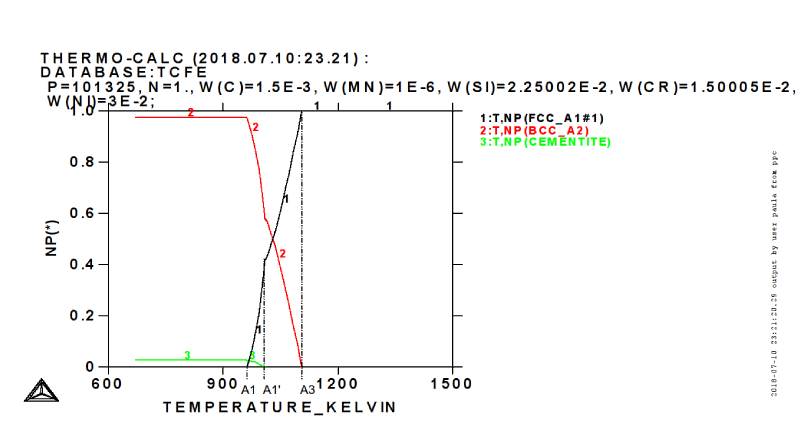
\includegraphics[width=.9\textwidth]{img/714editado.png}
  \caption{Extração de temperaturas críticas para aço hipoeutetóide}
  \label{fig:Tcrit_liga_hipo}
\end{figure}

\begin{figure}
  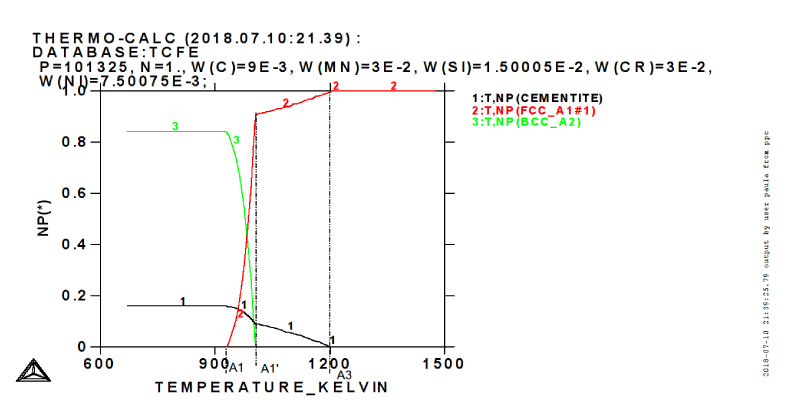
\includegraphics[width=.9\textwidth]{img/4321editado.png}
  \caption{Extração de temperaturas críticas para aço hipereutetóide}
  \label{fig:Tcrit_liga_hiper}
\end{figure}

\begin{figure}
  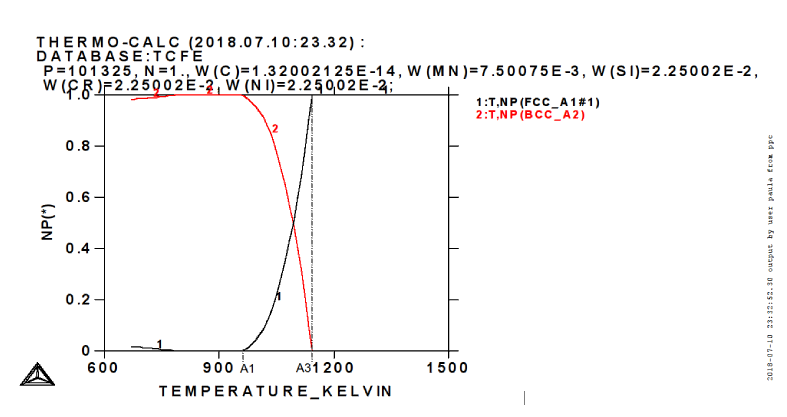
\includegraphics[width=.9\textwidth]{img/418editado.png}
  \caption{Extração de temperaturas críticas para aço hipoeutetóide sem cementita}
  \label{fig:Tcrit_liga_sem_cementita}
\end{figure}

A temperatura A1' é representada pela mudança de inclinação na curva da porcentagem de austenita. Para aços hipoeutetóides, essa temperatura corresponde ao ponto em que a porcentagem de cementita é zero, como mostra a Figura \ref{fig:Tcrit_liga_hipo}. Já para hipereutetóides, ao ponto em que a porcentagem de ferrita é zero, como na Figura \ref{fig:Tcrit_liga_hiper}. Enquanto isso, para aços em que a porcentagem de cementita é sempre zero, considera-se que a temperatura A1' é igual à A1 (vide Figura \ref{fig:Tcrit_liga_sem_cementita}).

É importante destacar que nem sempre um aço terá as três temperaturas críticas. Elementos muito alfagênicos podem não ter A3, como no caso de um $\gamma$ loop, e gamagênicos podem não ter A1, por terem austenita estável à temperatura ambiente.

Mesmo considerando que algumas temperaturas críticas podem não existir para certas composições, ainda está em estudo os erros que ocorreram nessa extração. Por exemplo, algumas composições com baixo carbono ficaram com valores em branco, enquanto outras tiveram valores de temperatura crítica muito acima do esperado, embora os gráficos plotados para sua respectiva composição estivessem dentro do esperado. Pretende-se corrigir esses erros antes dos resultados serem utilizados em um algoritmo de aprendizado de máquina.
Também foi realizada uma comparação dos valores de temperatura crítica com a equação empírica de Andrews, plotando o gráfico da Figura \ref{fig:tcrit_andrews}. A linha em azul representa os valores esperados ($T_{empirical} = T_{database}$).

\begin{figure}
  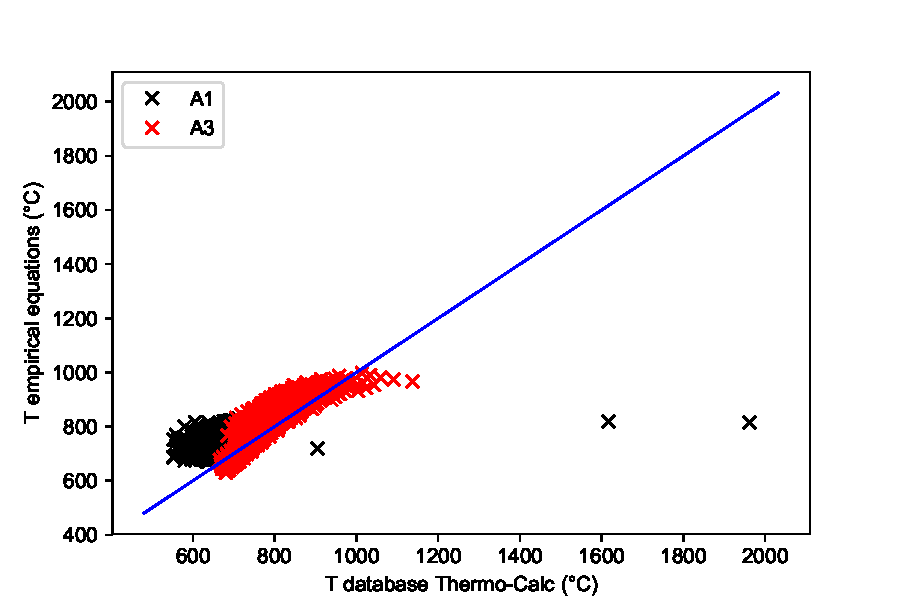
\includegraphics[width=1.1\textwidth]{img/andrews.pdf}
  \caption{Gráfico de temperatura crítica calculada pela equação empírica de Andrews e temperatura crítica do banco de dados}
  \label{fig:tcrit_andrews}
\end{figure}

Nota-se que, para as temperaturas A3, existe uma correlação maior com os valores calculados pela equação empírica, enquanto para A1 existe uma divergência maior. Isso pode estar relacionado a erros no script que extrai a temperatura A1, que ainda está em revisão. Outro fator que influencia na divergência é o fato de a equação de Andrews não ter membros interdependentes entre os elementos químicos, o que na prática não se aplica.

Para averiguar essa interdependência, plotou-se as isopletas de temperatura para cada elemento, variando a composição de carbono. Para cada elemento de liga, plotou-se cinco curvas, correspondentes aos cinco níveis de composição escolhidos.

Para o manganês e níquel, nota-se que a baixas concentrações de carbono a concentração do elemento de liga tem muita interferência no valor das temperaturas de transformação. A partir de 0,8\% C, as temperaturas são mais próximas para todos os níveis. Uma possível explicação é que os três elementos são gamagênicos.

Já para elementos alfagênicos, como o cromo, a relação se inverte. Para baixas concentrações de carbono, os valores de temperatura ficam próximos, e a partir de 0,4\% de carbono a concentração do cromo já contribui para sua divergência.

Um caso intermediário é o do silício, que apesar de alfagênico, tem influência na temperatura tanto a baixas quanto a mais altas concentrações de carbono, embora a influência a baixas concentrações seja maior.

\chapter{Conclusões parciais}

Até o momento o foram realizadas as etapas de simulações termodinâmicas e as rotinas para extração das temperaturas críticas foram implementadas com sucesso, de modo que o banco de dados que alimentará os algoritmos de aprendizado de máquina já foi construído. A comparação dos dados das temperaturas com equações empíricas para predição das temperaturas A1 e A3 mostra que, embora qualitativamente tanto os dados obtidos no presente trabalho quanto as equações da literatura apresentem tendências semelhantes, quantitativamente a correlação não é precisa.

\chapter{Próximas etapas}

Nas próximas etapas do trabalho serão implementados os algoritmos de aprendizado de máquina para predição das temperaturas críticas, a citar, redes neurais e regressão multivariável. O efeito dos elementos de liga nas temperaturas críticas serão avaliados com base nos parâmetros de ajuste dos algoritmos, como, por exemplo, os coeficientes de regressão.

\bibliography{tcc}

% \anexo{Composição química de aços de engenharia}
% \label{an:composicao}

\anexo{Diagramas binários}
\label{an:diag_bin}

\begin{figure}
  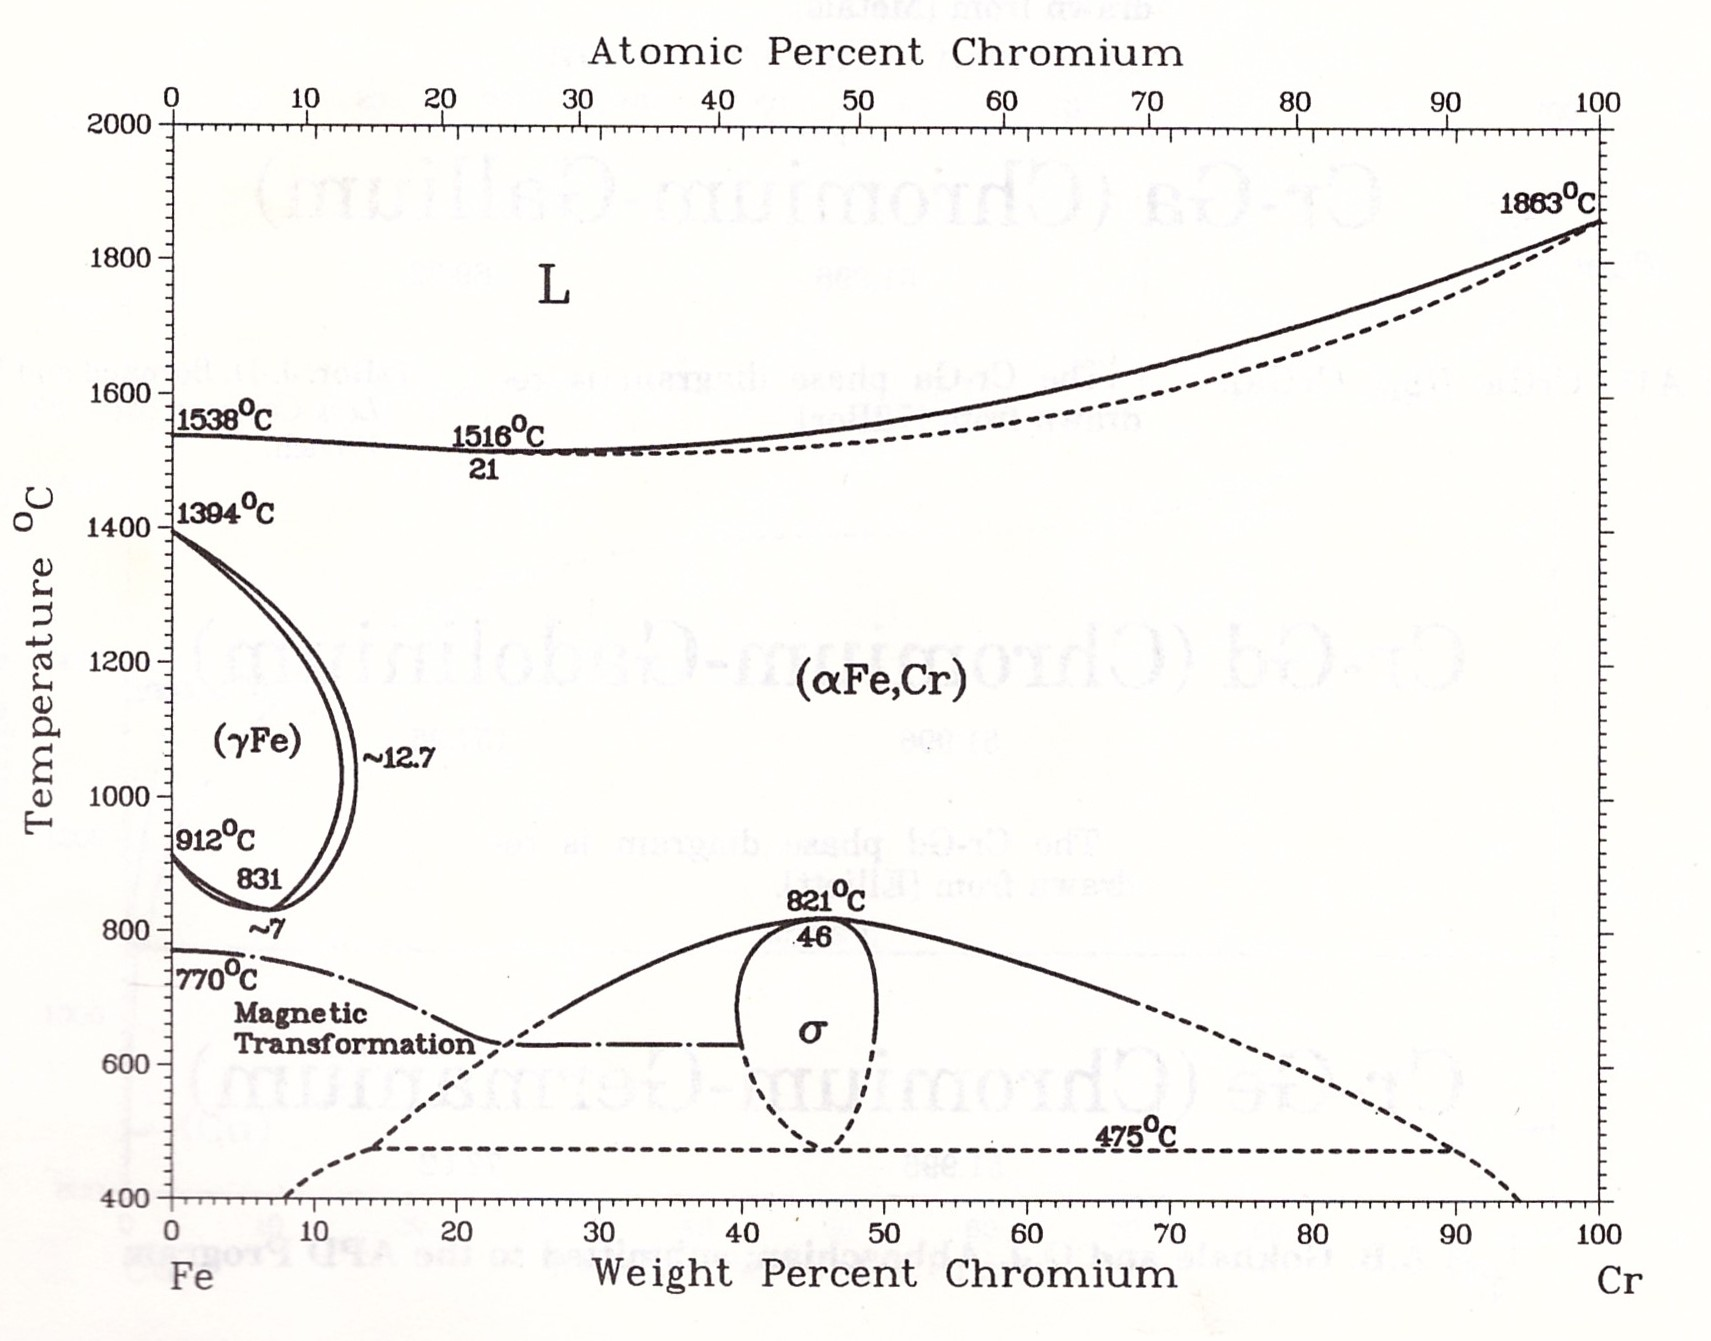
\includegraphics[width=1.1\textwidth]{img/Fe-Cr.jpg}
  \caption{Diagrama binário Fe-Cr}
  \label{fig:bin_fe-cr}
\end{figure}

\begin{figure}
  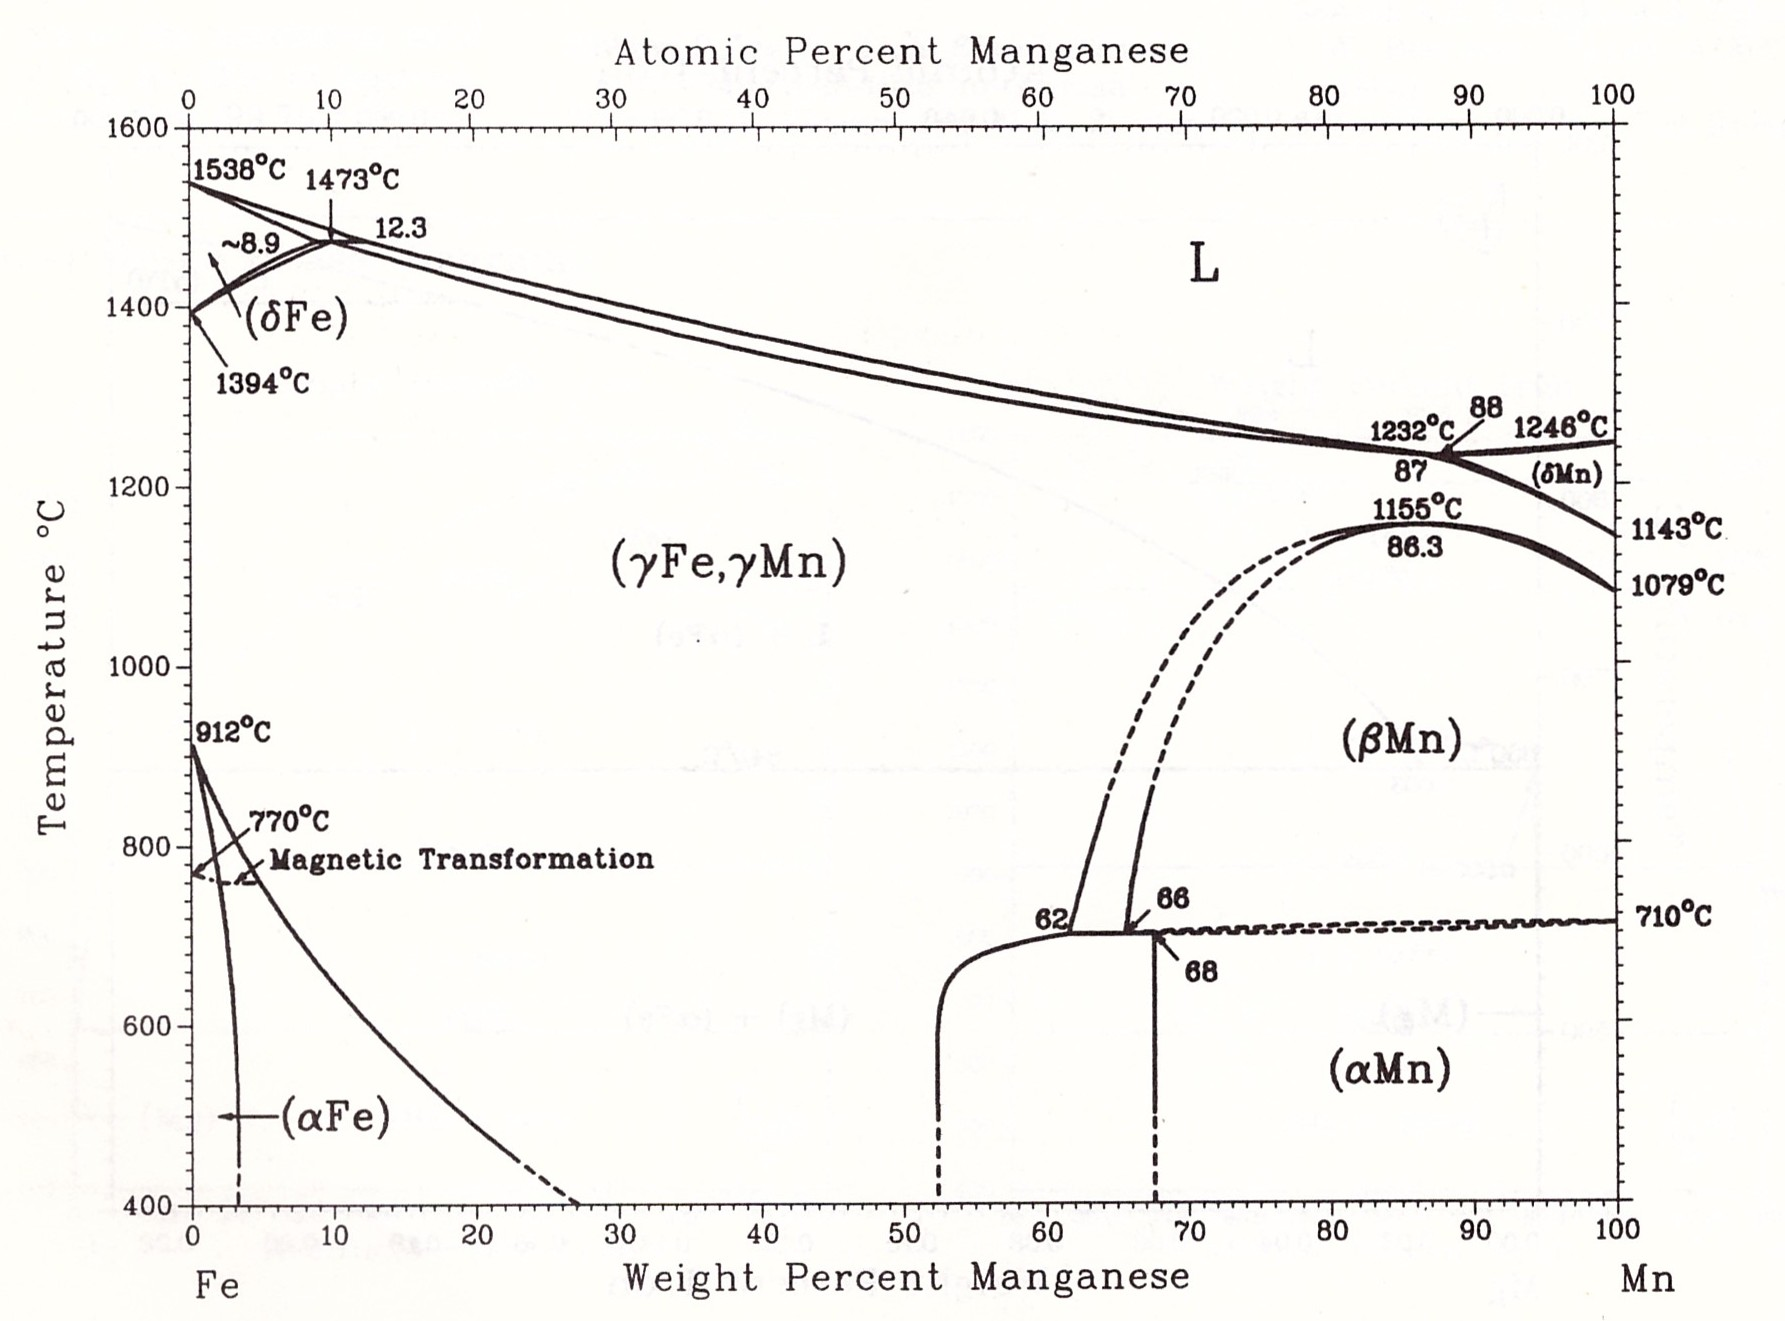
\includegraphics[width=1.1\textwidth]{img/Fe-Mn.jpg}
  \caption{Diagrama binário Fe-Mn}
  \label{fig:bin_fe-mn}
\end{figure}

\begin{figure}
  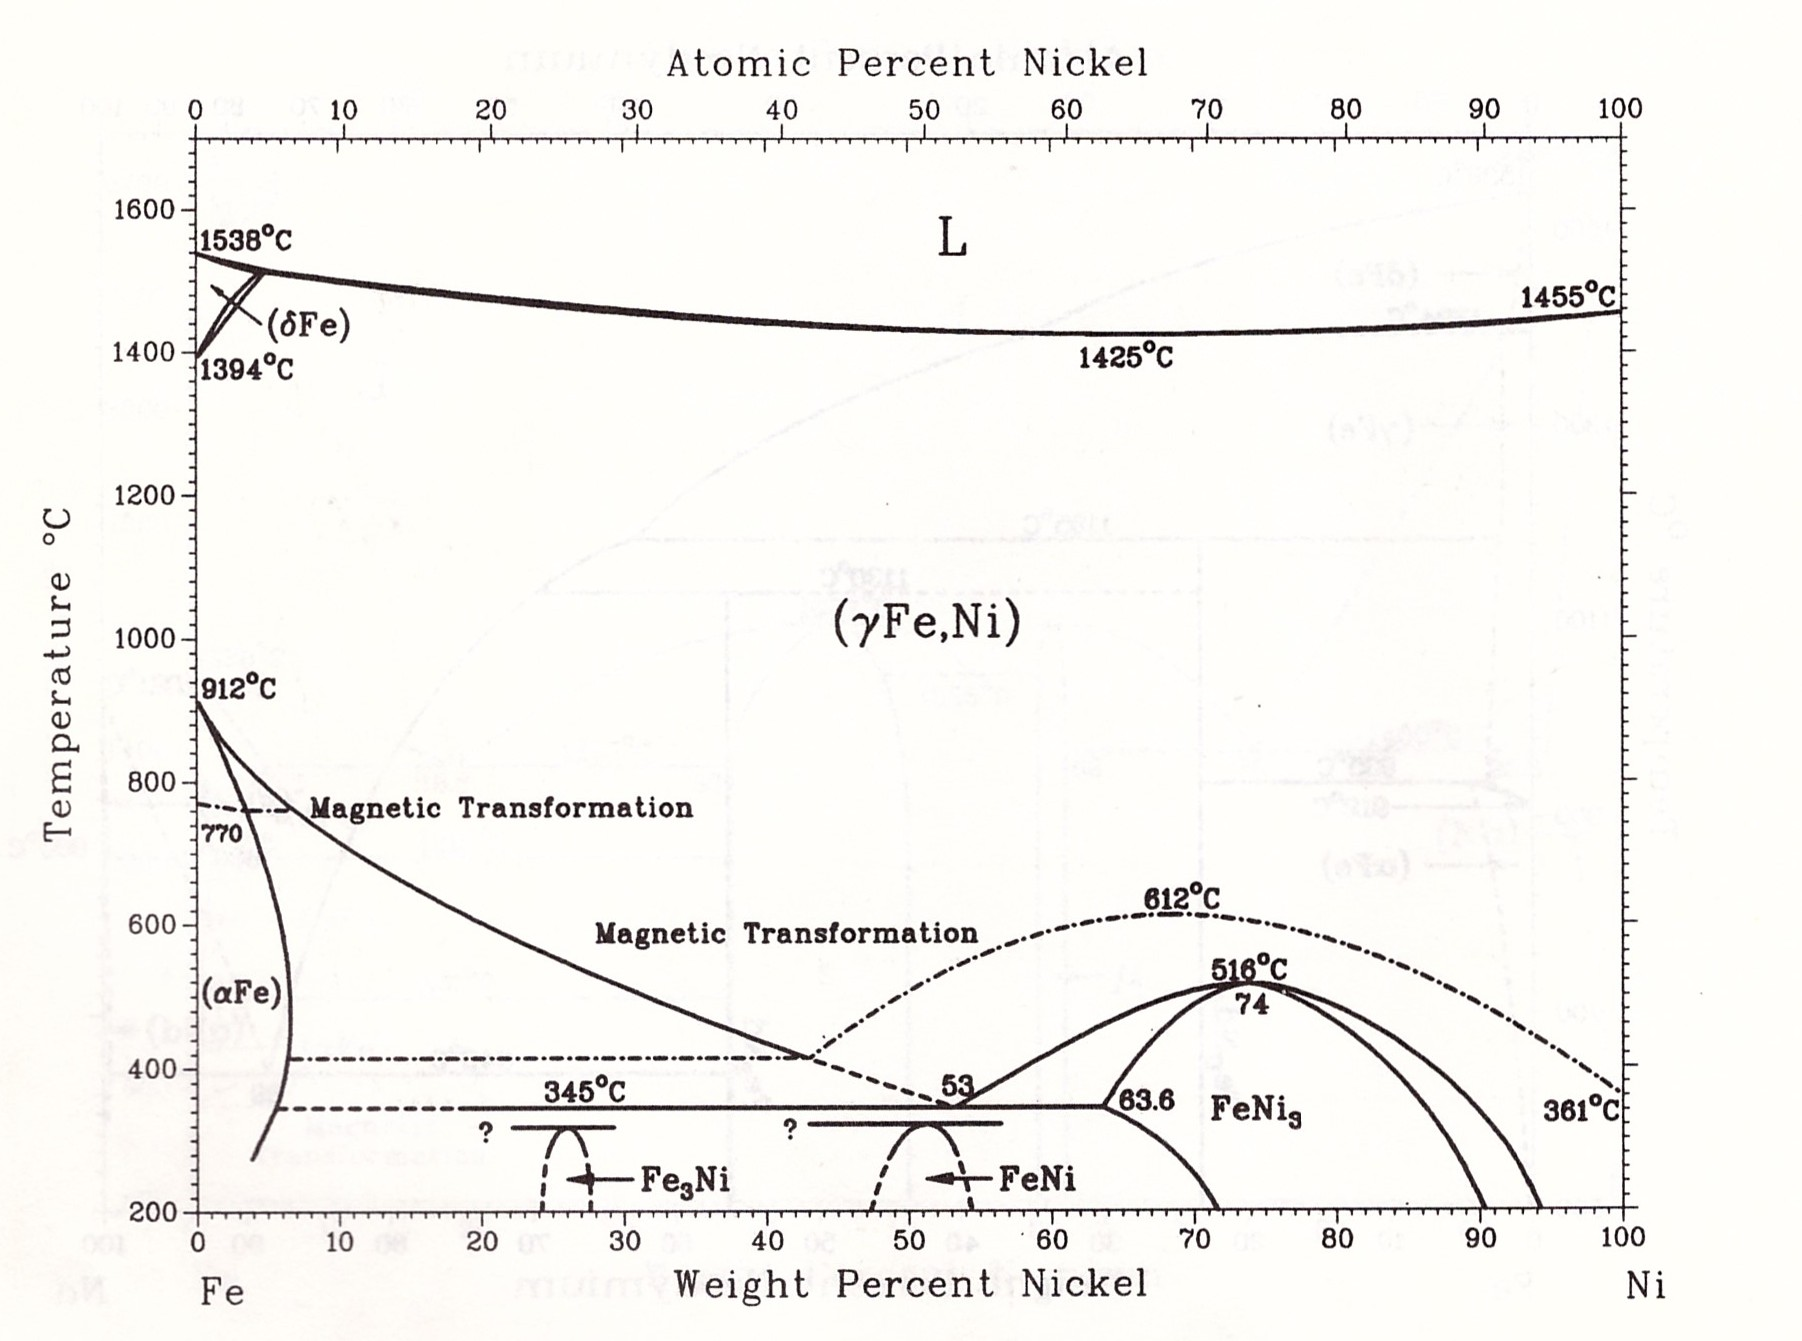
\includegraphics[width=1.1\textwidth]{img/Fe-Ni.jpg}
  \caption{Diagrama binário Fe-Ni}
  \label{fig:bin_fe-ni}
\end{figure}

\begin{figure}
  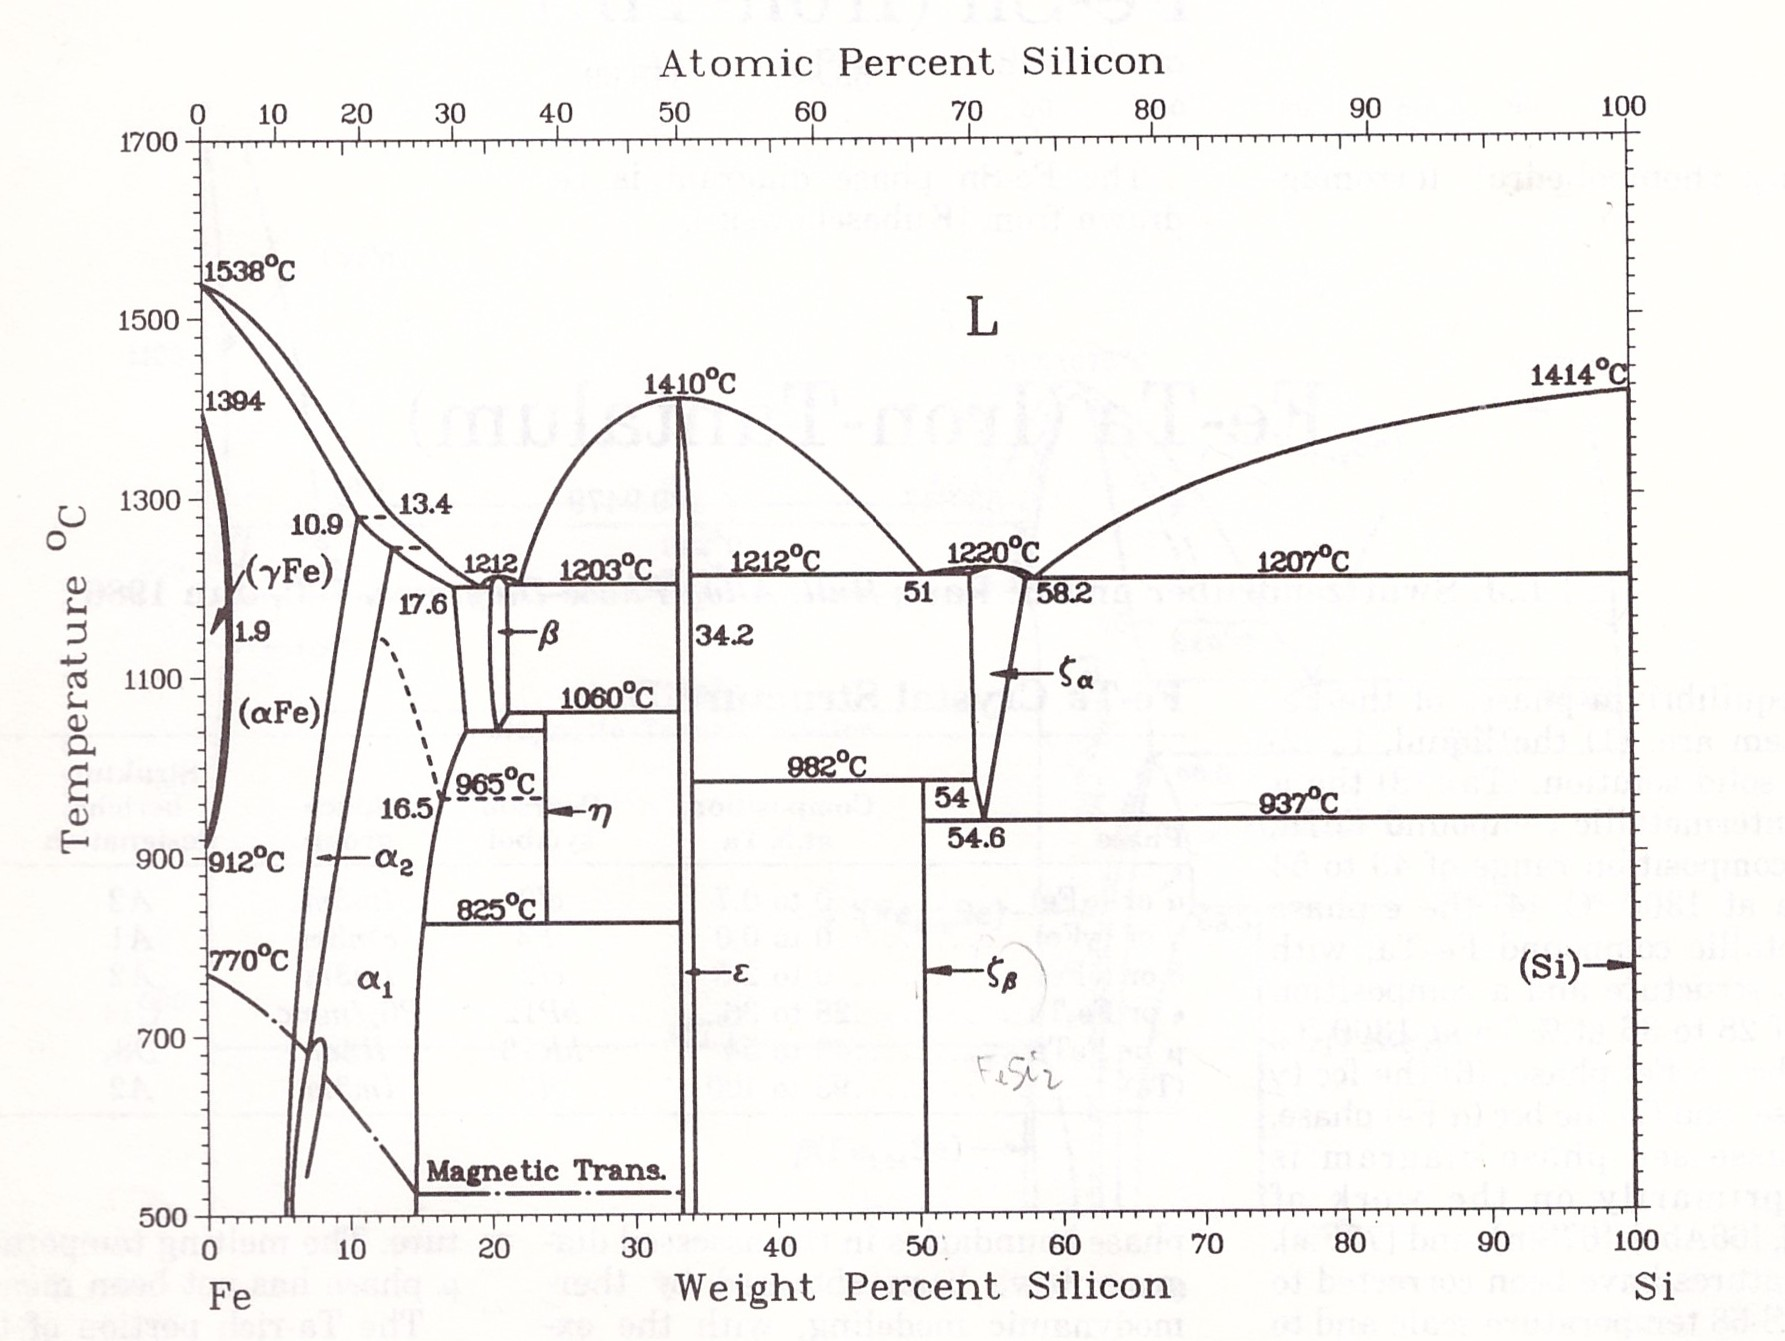
\includegraphics[width=1.1\textwidth]{img/Fe-Si.jpg}
  \caption{Diagrama binário Fe-Si}
  \label{fig:bin_fe-si}
\end{figure}

\end{document}
